%\ifx\wholebook\relax\else
%\documentclass[twoside]{book}
%\usepackage[active]{srcltx}
%\usepackage[LY1]{fontenc}
%\usepackage{url}
\makeatletter
\def\url@leostyle{%
  \@ifundefined{selectfont}{\def\UrlFont{\sf}}{\def\UrlFont{\sffamily}}}
\makeatother
% Now actually use the newly defined style.
\urlstyle{leo}

\usepackage{graphicx}
\def\etc{{\textit{etc}}}
\def\eg{{\textit{e.g.}}}
\def\ie{{\textit{i.e.}}}
\def\cf{{\textit{c.f.}}\ }
\def\erf{\mathop{\textrm{erf}}}
\def\sign{\mathop{\textrm{sign}}}
\def\prob{\mathop{\textrm{Prob}}}
\def\var{\mathop{\textrm{var}}}
\def\mod{\mathop{\textrm{mod}}}
\def\cor{\mathop{\textrm{cor}}}
\def\cov{\mathop{\textrm{cov}}}
\def\cl{\mathop{\textrm{CL}}}
\def\kg{\mathop{\textrm{Kg}}}
\def\patstyle#1{{\textsc #1}}
\def\th{^{\mathop{\textrm{th}}}}
%\def\st#1{^{\mathop{\rm #1}}}
\def\note#1{\begin{quote}{\textbf{Note:}} #1\end{quote}}
\def\braket#1{\left\langle #1\right\rangle}
\def\order#1{\let\o=#1$\mathcal{O}$\ifx\o 1$\left(n\right)$\else$\left(n^{#1}\right)$\fi}
%\newtheorem{privListing}{Listing}[chapter]
%\newenvironment{listing}{\vskip 3ex\hrule\vskip 1ex\begin{privListing}}{\end{privListing}\hrule\vskip 1ex}
\newtheorem{privExample}{Code example}[chapter]
\newenvironment{codeExample}{\begin{privExample}\begin{quote}\tt}{\end{quote}\end{privExample}}
\def\relboxl#1#2{\hbox to #1\hsize{#2\hfil}}
\def\relboxc#1#2{\hbox to #1\hsize{\hfil #2\hfil}}
\def\relboxr#1#2{\hbox to #1\hsize{\hfil #2}}
\def\transpose#1{\textbf{#1}^{\mathop\textrm{T}}}
\def\inverse#1{\textbf{#1}^{-1}}
%\def\tm{$^{\mathop{\rm TM}}$}
\def\tm{ }
\newenvironment{mainEquation}{\marginpar[\vspace{3 ex} Main
equation$\Rightarrow$]{\vspace{3 ex}$\Leftarrow$Main
equation}\begin{equation}}{\end{equation}}
\def\rubrique#1{\paragraph{#1}\hfil\par\noindent}

%\begin{document}
%\fi

\chapter{Elements of statistics}
\label{ch:statistics} \vspace{1 ex}
\begin{flushright} {\textsl La statistique est la premi\`ere des sciences inexactes.}\footnote{Statistics is the first of the inexact sciences.}\\
Edmond et Jules de Goncourt
\end{flushright}
\vspace{1 ex} Statistical analysis comes into play when dealing
with a large amount of data. Obtaining information from the
statistical analysis of data is the subject of chapter
\ref{ch:estimation}. Some sections of chapter \ref{ch:datamining}
are also using statistics. Concepts needed by statistics are based
on probability theory.

This chapter makes a quick overview of the concepts of probability
theory. It is the third (and last) chapter of this book where most
of the material is not useful {\textit per se}.
Figure \ref{fig:statisticsclasses} shows the classes described in this
chapter.
\begin{figure}
\centering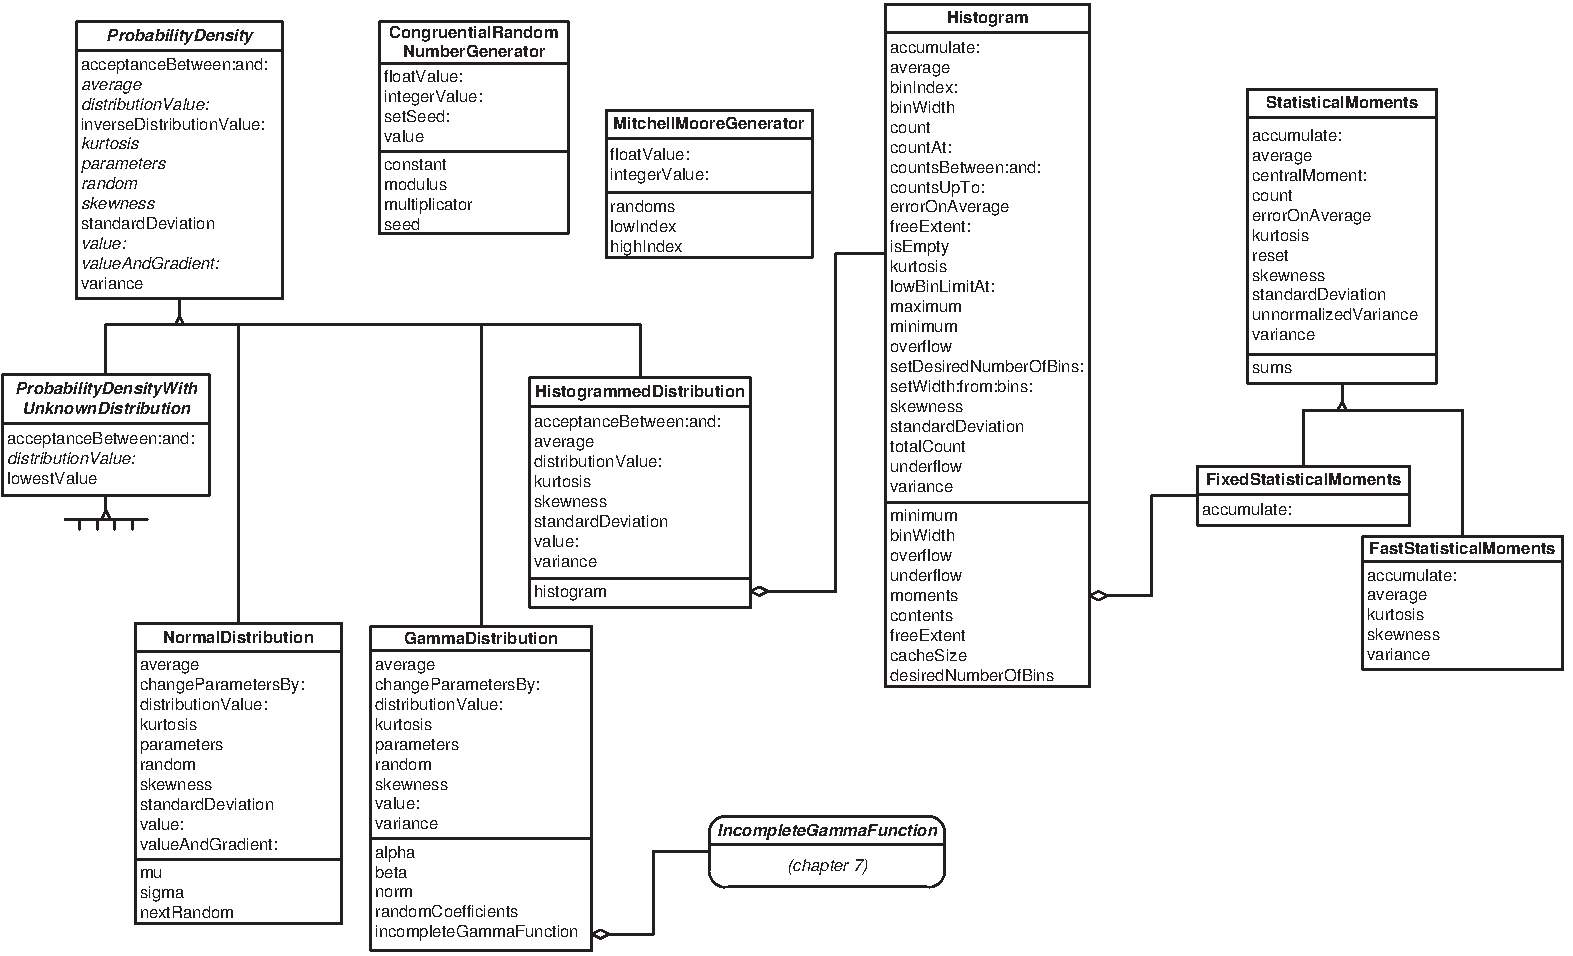
\includegraphics[width=11cm]{Figures/StatisticsClasses}
\caption{Classes related to statistics}
\label{fig:statisticsclasses}
\end{figure}
All these classes, however, are used extensively in the remaining
chapters of this book. The example on how to use the code are kept
to a minimum since real examples of use can be found in the next
chapters.

An in-depth description of probability theory is beyond the scope
of this book. The reader in the need for additional should consult
the numerous textbooks on the subject, \cite{PhiTay} or
\cite{LawKel} for example.

\section{Statistical moments}
\label{sec:moments} When one measures the values of an observable
random variable, each measurement gives a different magnitude.
Assuming measurement errors are negligible, the fluctuation of the
measured values correspond to the distribution of the random
variable. The problem to be solved by the experimenter is to
determine the parameters of the distribution from the observed
values. {\textsl Statistical moments} can contribute to the
characterization of the distribution\footnote{Central moments are
related to the coefficients of the Taylor expansion of the Fourier
transform of the distribution function.}.

Given a set of measurements, $x_1,\ldots,x_n$, of the values
measured for a random variable one defines the moment of $k\th$
order by:
\begin{equation}
  M_k={1\over n}\sum_{i=1}^n x_i^k.
\end{equation}
In particular, the moment of first order is the mean or average of
the set of data:
\begin{equation}
\label{eq:average}
  \bar{x}=M_1={1\over n}\sum_{i=1}^n x_i.
\end{equation}
The central moments of $k^{\mathop{\textrm th}}$ order is defined by:
\begin{equation}
  m_k={1\over n}\sum_{i=1}^n \left(x_i-\bar{x}\right)^k.
\end{equation}
where $k$ is larger than 1. The central moments are easily
expressed in terms of the moments. We have:
\begin{equation}
  m_k=\sum_{j=0}^k \left({k \atop j}\right)\left(-\bar{x}\right)^{k-j}M_j,
\end{equation}
where $\left({k \atop j}\right)$ are the binomial coefficients.

Some statistical parameters are defined on the central moments.
The variance of a set of measurement is the central moment of
second order. The standard deviation, $s$, is the square root of
the variance given by the following formula:
\begin{equation}
s^2={\displaystyle n \over \displaystyle n-1}m_2 ={\displaystyle 1
\over \displaystyle n-1} \sum_{i=1}^n \left(x_i-\bar{x}\right)^2.
\end{equation}
The factor in front the central moment of second order is called
Bessel's correction factor. This factor removes the bias of the
estimation when the standard deviation is evaluated over a finite
sample. The standard deviation measures the spread of the data
around the average.

Many people believe that the standard deviation is the error of
the average. This is not true: the standard deviation describes
how much the data are spread around the average. It thus
represents the error of a single measurement. An estimation of the
standard deviation of the average value is given by the following
formula:
\begin{equation}
\label{eq:averagerror}
  s_{\bar{x}}^2={\displaystyle s^2 \over n}
  \mbox{\quad or \quad}
  s_{\bar{x}}={\displaystyle s \over \sqrt{n}}.
\end{equation}
This expression must be taken as the error on the average when
performing a least square fit on averaged data, for example.

Two quantities are related to the central moments of $3\st{rd}$
and $4\th$ order. Each of these quantities are normalized by the
adequate power of the standard deviation needed to yield a
quantity without dimension.

\noindent The skewness is defined by:
\begin{equation}
  a={\displaystyle n \over\displaystyle
  \left(n-1\right)\left(n-2\right)s^3}m_3
  ={\displaystyle 1 \over\displaystyle
  \left(n-1\right)\left(n-2\right)}
  \sum_{i=1}^n\left({\displaystyle x_i-\bar{x}\over\displaystyle s}\right)^3.
\end{equation}
The skewness is a measure of the asymmetry of a distribution. If
the skewness is positive, the observed distribution is asymmetric
toward large values and vice-versa.

\noindent The kurtosis is defined by
\begin{equation}
\label{eq:kurtosis}
  \begin{array}{rl}
    k=& {\displaystyle n\left(n+1\right) \over\displaystyle
  \left(n-1\right)\left(n-2\right)\left(n-3\right)s^4}m_4 -{\displaystyle 3\left(n-1\right)^2 \over\displaystyle
  \left(n-2\right)\left(n-3\right)}\\*[2ex]
    =& {\displaystyle \left(n+1\right) \over\displaystyle
  \left(n-1\right)\left(n-2\right)\left(n-3\right)}
  \displaystyle\sum_{i=1}^n\left({\displaystyle x_i-\bar{x}\over\displaystyle s}\right)^4 -{\displaystyle 3\left(n-1\right)^2 \over\displaystyle
  \left(n-2\right)\left(n-3\right)}
  \end{array}
\end{equation}
The kurtosis is a measure of the peakedness or flatness of a
distribution in the region of the average. The subtracted term in
equation \ref{eq:kurtosis} is a convention defining the kurtosis
of the normal distribution as 0\footnote{One talks about a {\textsl
platykurtic} distribution when the kurtosis is negative, that is
the peak of the distribution is flatter than that of the normal
distribution. Student (\cf section \ref{sec:ttest}) and Cauchy
(\cf section \ref{sec:cauchydist}) distributions are platykurtic.
The opposite is called {\textsl leptokurtic}. The Laplace (\cf section
\ref{sec:laplacedist}) distribution is leptokurtic. }.

As we have seen, the average, standard deviation, skewness and
kurtosis are parameters, which helps characterizing a distribution
of observed values. To keep track of these parameters, it is handy
to define an object whose responsibility is to accumulate the
moments up to order 4. One can then easily compute the parameters
of the distribution. It can be used in all cases where
distribution parameters are needed.

\subsection{Statistical moments --- Smalltalk implementation}
\marginpar{Figure \ref{fig:statisticsclasses} with the box {\textbf
FastStatisticalMoments} grayed.} To describe this implementation
we must anticipated on the next section: the class {\textbf
FastStatisticalMoments} implementing statistical moments as
described in Section \ref{sec:moments} is a subclass of the class
defined in section \ref{sec:robustmoment}.

Space allocation is handled by the superclass. The class {\texttt
FastStatisticalMoments} uses this allocation to store the moments
(instead of the central moments). The method {\texttt accumulate:}
perform the accumulation of the moments. The methods {\texttt
average}, {\texttt variance}, {\texttt skewness} and {\texttt kurtosis}
compute the respective quantities using explicit expansion of the
central moments as a function of the moments.

The computation of the standard deviation and of the error on the
average are handled by the superclass (\cf listing
\ref{ls:genmoments}).

\label{sec:smoments}Listing \ref{lst:fastmoments} shows the
Smalltalk implementation. The class {\texttt
PMFastStatisticalMoments} is a subclass of class {\texttt
PMStatisticalMoments} presented in listing \ref{lst:genmoments} of
section \ref{sec:srobustmoment}. The reason for the split into two
classes will become clear in section \ref{sec:robustmoment}.

The following code shows how to use the class {\texttt
PMFastStatisticalMoments} to accumulate measurements of a random
variable and to extract the various distribution parameters
discussed in section \ref{sec:moments}.

\begin{displaycode}{Smalltalk}
| accumulator valueStream average stdev skewness kurtosis |
accumulator := PMFastStatisticalMoments new.
[ valueStream atEnd ]
        whileFalse: [ accumulator accumulate: valueStream next ].
average := accumulator average.
stdev := accumulator standardDeviation.
skewness := accumulator skewness.
kurtosis := accumulator kurtosis
\end{displaycode}

This example assumes that the measurement of the random variable
are obtained from a stream. The exact implementation of the stream
is not shown here.

After the declarative statements, the first executable statement
creates a new instance of the class {\texttt
PMFastStatisticalMoments} with the default dimension. This
default allocates enough storage to accumulate up to the moment of
$4\th$ order. The next two lines are the accumulation proper using
a {\texttt whileFalse:} construct and the general behavior of a
stream. The last four lines extract the main parameters of the
distribution.

If any of the distribution's parameters --- average, variance,
skewness or kurtosis --- cannot be computed, the returned value is
{\texttt nil}.

\begin{listing}[label=lst:fastmoments]{Smalltalk}
{Smalltalk fast implementation of statistical moments}
PMStatisticalMoments subclass: #PMFastStatisticalMoments
   instanceVariableNames: ''
   classVariableNames: ''
   package: 'Math-StatisticalMoments'
\end{listing}

\begin{displaycode}{Smalltalk}
PMFastStatisticalMoments >> accumulate: aNumber
    | var |
    var := 1.
    1 to: moments size
        do: 
            [ :n | 
            moments at: n put: (moments at: n) + var.
            var := var * aNumber ]
\end{displaycode}

\begin{displaycode}{Smalltalk}
PMFastStatisticalMoments >> average
    self count = 0 ifTrue: [ ^nil ].
    ^ (moments at: 2) / self count
\end{displaycode}

\begin{displaycode}{Smalltalk}
PMFastStatisticalMoments >> kurtosis
    | var x1 x2 x3 x4 kFact kConst n m4 xSquared |
    n := self count.
    n < 4 ifTrue: [^nil].
    var := self variance.
    var = 0 ifTrue: [^nil].
    x1 := (moments at: 2) / n.
    x2 := (moments at: 3) / n.
    x3 := (moments at: 4) / n.
    x4 := (moments at: 5) / n.
    xSquared := x1 squared.
    m4 := x4 - (4 * x1 * x3) + (6 * x2 * xSquared) - (xSquared 
                                                         squared * 3).
    kFact := n * (n + 1) / (n - 1) / (n - 2) / (n - 3).
    kConst := 3 * (n - 1) * (n - 1) / (n - 2) / (n - 3).
    ^ kFact * (m4 * n / var squared) - kConst
\end{displaycode}

\begin{displaycode}{Smalltalk}
PMFastStatisticalMoments >> skewness
    | x1 x2 x3 n stdev |
    n := self count.
    n < 3 ifTrue: [ ^nil ].
    stdev := self standardDeviation.
    stdev = 0 ifTrue: [^nil].
    x1 := (moments at: 2) / n.
    x2 := (moments at: 3) / n.
    x3 := (moments at: 4) / n.
    ^ (x3 - (3 * x1 * x2) + (2 * x1 * x1 * x1)) * n * n 
        / (stdev squared * stdev * (n - 1) * (n - 2))
\end{displaycode}

\begin{displaycode}{Smalltalk}
PMFastStatisticalMoments >> variance
    | n |
    n := self count.
    n < 2 ifTrue: [^nil].
    ^ ((moments at: 3) - ((moments at: 2) squared / n)) / (n - 1)
\end{displaycode}

\section{Robust implementation of statistical moments}
\label{sec:robustmoment} The methods used to implement the
computation of the central moments in the previous section is
prone to rounding errors. Indeed, contribution from values distant
from the average can totally offset a result, however infrequent
they are. Such an effect is worse when the central moments are
derived from the moments. This section gives an algorithm ensuring
minimal rounding errors.

The definition of statistical moments is based on the concept of
expectation value. The expectation value is a linear operator over
all functions of the random variable. If one measures the values
of the random variable $n$ times, the expectation value of a
function $f\left(x\right)$ of a random variable $x$ is estimated
by the following expression:
\begin{equation}
\label{eq:expectation}
 \left\langle f\left(x\right)\right\rangle_n
= {1\over n}\sum_{i=1}^n f\left(x_i\right),
\end{equation}
where the values $x_1,\ldots,x_n$ are the measurements of the
random variable. A comparison of equation \ref{eq:expectation}
with \ref{eq:average} shows that the average is simply the
expectation value of the function $f\left(x\right)=x$. The central
moment of order $k$ is the expectation value of the function
$\left(x-\bar{x}\right)^k$:
\begin{equation}
\label{eq:expectmoment}
 \left\langle \left(x-\bar{x}\right)^k\right\rangle_n
= {1\over n}\sum_{i=1}^n \left(x_i-\bar{x}\right)^k.
\end{equation}

To miminize rounding errors, one computes the changes occurring to
the central moments when a new value is taken into account. In
other words, one computes the value of a central moment over $n+1$
values as a function of the central moment over $n$ values and the
$\left(n+1\right)\th$ value. For the average, we have
\begin{equation}
\label{eq:accumaverage}
  \begin{array}{ll}
 \left\langle x\right\rangle_{n+1}
   &= \displaystyle{1\over n+1}\sum_{i=1}^{n+1} x_i\\
   &=\displaystyle {x_{n+1}\over n+1}+{1\over n+1}\sum_{i=1}^n x_i\\
   &=\displaystyle {x_{n+1}\over n+1}+{n\over n+1}\left\langle x\right\rangle_n\\
   &=\displaystyle {x_{n+1}\over n+1}+\left(1-{1\over n+1}\right)\left\langle x\right\rangle_n\\
   &=\displaystyle\left\langle x\right\rangle_n- {\left\langle x\right\rangle_n-x_{n+1}\over
   n+1}.
  \end{array}
\end{equation}
Thus, the estimator of the average over $n+1$ measurements can be
computed from the estimator of the average over $n$ measurements
by subtracting a small correction, $\Delta_{n+1}$, given by:
\begin{mainEquation}
\label{eq:deltaverage}
  \begin{array}{ll}
    \Delta_{n+1}&=\displaystyle\left\langle x\right\rangle_n - \left\langle
    x\right\rangle_{n+1}\\
    &=\displaystyle{\left\langle x\right\rangle_n-x_{n+1}\over
    n+1}.
  \end{array}
\end{mainEquation}
The expression in the numerator of equation \ref{eq:deltaverage}
subtracts two quantities of comparable magnitude. This ensures a
minimization of the rounding errors.

A similar derivation can be made for the central moments of higher
orders. A complete derivation is given in appendix
\ref{sec:centralmoments}. The final expression is
\begin{mainEquation}
\label{eq:deltamoment}
  \left\langle\left(x-\bar{x}\right)^k\right\rangle_{n+1}
  ={n\over n+1}\left\{
  \left[ 1 - \left(-n\right)^{k-1}\right]\Delta_{n+1}^k
  +\sum_{l=2}^k \left({l\atop k}\right)
  \left\langle\left(x-\mu\right)^l\right\rangle_n
  \Delta_{n+1}^{k-l}
  \right\}.
\end{mainEquation}
The reader can verify the validity of equation
\ref{eq:deltamoment} by verifying that it gives 1 for $k=0$ and 0
for $k=1$. Put in this form, the computation of the central moment
estimators minimizes indeed rounding errors. For the central
moment of order 2 we have:
\begin{mainEquation}
\label{eq:accumvariance}
  \left\langle\left(x-\bar{x}\right)^2\right\rangle_{n+1}
  ={n\over n+1}\left\{
  \left(1+n\right)\Delta_{n+1}^2
  +\left\langle\left(x-\bar{x}\right)^2\right\rangle_n
  \right\}.
\end{mainEquation}
For the central moment of order 3 we have:
\begin{mainEquation}
\label{eq:accumskewness}
  \left\langle\left(x-\bar{x}\right)^3\right\rangle_{n+1}
  ={n\over n+1}\left\{
  \left(1-n^2\right)\Delta_{n+1}^3
  +3\left\langle\left(x-\bar{x}\right)^2\right\rangle_n\Delta_{n+1}
  +\left\langle\left(x-\bar{x}\right)^3\right\rangle_n
  \right\}.
\end{mainEquation}
For the central moment of order 4 we have:
\begin{mainEquation}
\label{eq:accumkurtosis}
  \begin{array}{ll}
  \left\langle\left(x-\bar{x}\right)^4\right\rangle_{n+1}
  =\displaystyle{n\over n+1}&\left\{
  \left(1+n^3\right)\Delta_{n+1}^4
  +6\left\langle\left(x-\bar{x}\right)^2\right\rangle_n\Delta_{n+1}^2\right.\\
  &\left.+4\left\langle\left(x-\bar{x}\right)^3\right\rangle_n\Delta_{n+1}
  +\left\langle\left(x-\bar{x}\right)^4\right\rangle_n
  \right\}.
  \end{array}
\end{mainEquation}

\subsection{Robust central moments --- General implementation}
\marginpar{Figure \ref{fig:statisticsclasses} with the boxes {\textbf
StatisticalMoments} and {\textbf FixedStatisticalMoments} grayed.} The
class {\texttt StatisticalMoments} has a single instance variable {\texttt
moments} used to store the accumulated central moments.

The evaluation of equation \ref{eq:deltamoment} is not as hard as
it seems from a programming point of view. One must remember that
the binomial coefficients can be obtained by recursion (Pascal
triangle). Furthermore, the terms of the sum can be computed
recursively from those of the previous order so that raising the
correction $\Delta_{n+1}$ to an integer power is never made
explicitly. Equation \ref{eq:deltamoment} is implemented in method
{\texttt accumulate}. The reader will notice that the binomial
coefficients are computed inside the loop computing the sum.

Accumulating the central moments using equation
\ref{eq:deltamoment} has the advantage that the estimated value of
the central moment is always available. Nevertheless, accumulation
is about 2 times slower than with the brute force method exposed
in section \ref{sec:moments}. The reader must decide between speed
and accuracy to chose between the two implementations.

The class {\texttt FixedStatisticalMoments} is a subclass of class
{\texttt StatisticalMoments} specialized in the accumulation of
central moments up to order 4. Instead of implementing the general
equation \ref{eq:deltamoment}, the central moments are accumulated
using equations \ref{eq:accumvariance}, \ref{eq:accumskewness} and
\ref{eq:accumkurtosis}. The only instance method redefined by this
class is the method {\texttt accumulate}. All other computations are
performed using the methods of the superclass.

\subsection{Robust central moments --- Smalltalk implementation}
\label{sec:srobustmoment} Listing
\ref{ls:genmoments} shows the implementation of the robust
statistical moments. Listing \ref{lst:fixedmoments} shows a
specialization to optimize the speed of accumulation for the most
frequently used case (accumulation up to the $4\th$ order).

Using the class is identical for all classes of the hierarchy.
Thus, the code example presented in section \ref{sec:smoments} is
also valid for these two classes.

The creation method {\texttt new:} takes as argument the highest order
of the accumulated moments. The corresponding initialization
method allocates the required storage. The creation method {\texttt
new} corresponds to the most frequent usage: the highest order is
4.

The methods computing the distribution parameters --- average,
variance, skewness and kurtosis --- are using the method {\texttt
centralMoment:} retrieving the central moment of a given order.
They will return {\texttt nil} if not enough data as been accumulated
in the moments.

\begin{listing}[label=lst:genmoments]{Smalltalk}
{Smalltalk implementation of accurate statistical moments}
Object subclass: #PMStatisticalMoments
   instanceVariableNames: 'moments'
   classVariableNames: ''
   package: 'Math-StatisticalMoments'
\end{listing}

\begin{displaycode}{Smalltalk}
PMStatisticalMoments class >> new
    ^ self new: 4
\end{displaycode}

\begin{displaycode}{Smalltalk}
PMStatisticalMoments class >> new: anInteger
    ^ super new initialize: anInteger + 1
\end{displaycode}

\begin{displaycode}{Smalltalk}
PMStatisticalMoments >> accumulate: aNumber
    | correction n n1 oldSums pascal nTerm cTerm term |
    n := moments at: 1.
    n1 := n + 1.
    correction := ((moments at: 2) - aNumber) / n1.
    oldSums := moments copyFrom: 1 to: moments size.
    moments
        at: 1 put: n1;
        at: 2 put: (moments at: 2) - correction.
    pascal := Array new: moments size.
    pascal atAllPut: 0.
    pascal
        at: 1 put: 1;
        at: 2 put: 1.
    nTerm := -1.
    cTerm := correction.
    n1 := n / n1.
    n := n negated.
    3 to: moments size
        do: 
            [:k | 
            cTerm := cTerm * correction.
            nTerm := n * nTerm.
            term := cTerm * (1 + nTerm).
            k to: 3
                by: -1
                do: 
                    [:l | 
                    pascal at: l put: (pascal at: l - 1) + (pascal 
                                                               at: l).
                    term := (pascal at: l) * (oldSums at: l) + term.
                    oldSums at: l put: (oldSums at: l) * correction ].
            pascal at: 2 put: (pascal at: 1) + (pascal at: 2).
            moments at: k put: term * n1 ]
\end{displaycode}

\begin{displaycode}{Smalltalk}
PMStatisticalMoments >> average
    self count = 0 ifTrue: [ ^nil ].
    ^ moments at: 2
\end{displaycode}

\begin{displaycode}{Smalltalk}
PMStatisticalMoments >> centralMoment: anInteger
    ^ moments at: anInteger + 1
\end{displaycode}

\begin{displaycode}{Smalltalk}
PMStatisticalMoments >> count
    ^ moments at: 1
\end{displaycode}

\begin{displaycode}{Smalltalk}
PMStatisticalMoments >> errorOnAverage
    ^ (self variance / self count) sqrt
\end{displaycode}

\begin{displaycode}{Smalltalk}
PMStatisticalMoments >> initialize: anInteger
    moments := Array new: anInteger.
    self reset.
    ^ self
\end{displaycode}

\begin{displaycode}{Smalltalk}
PMStatisticalMoments >> kurtosis
    | n n1 n23 |
    n := self count.
    n < 4 ifTrue: [^nil].
    n23 := (n - 2) * (n - 3).
    n1 := n - 1.
    ^ ((moments at: 5) * n squared * (n + 1) / (self variance squared 
                                                                * n1) 
        - (n1 squared * 3)) / n23
\end{displaycode}

\begin{displaycode}{Smalltalk}
PMStatisticalMoments >> reset
    moments atAllPut: 0
\end{displaycode}

\begin{displaycode}{Smalltalk}
PMStatisticalMoments >> skewness
    | n v |
    n := self count.
    n < 3 ifTrue: [^nil].
    v := self variance.
    ^ (moments at: 4) * n squared / ((n - 1) * (n - 2) * (v sqrt * v))
\end{displaycode}

\begin{displaycode}{Smalltalk}
PMStatisticalMoments >> standardDeviation
    ^ self variance sqrt
\end{displaycode}

\begin{displaycode}{Smalltalk}
PMStatisticalMoments >> unnormalizedVariance
    ^ (self centralMoment: 2) * self count
\end{displaycode}

\begin{displaycode}{Smalltalk}
PMStatisticalMoments >> variance
    | n |
    n := self count.
    n < 2
        ifTrue: [ ^nil].
    ^ self unnormalizedVariance / ( n - 1)
\end{displaycode}

The class {\texttt PMFixedStatisticalMoments} is a specialization of
the class {\texttt PMStatisticalMoments} for a fixed number of
central moments going up to the $4\th$ order.

The class creation method {\texttt new:} is barred from usage as the
class can only be used for a fixed number of moment orders. As a
consequence the default creation method must be redefined to
delegate the parametric creation to the method of the superclass.

\begin{listing} Smalltalk implementation of accurate statistical moments with fixed orders \label{ls:fixedmoments}
%$$\halign{ #\hfil&\quad#\hfil\cr {\sl Class}& {\Large\bf DhbFixedStatisticalMoments}\cr
{\sl Subclass of }&{\tt DhbStatisticalMoments}\cr\noalign{\vskip 1ex}
}$$


Class methods
{\parskip 1ex\par\noindent}
{\bf new}
\begin{verbatim}
    ^ super new: 4
\end{verbatim}
{\bf new:} {\tt anInteger}
\begin{verbatim}
    ^ self error: 'Illegal creation message for this class'
\end{verbatim}

Instance methods
{\parskip 1ex\par\noindent}
{\bf accumulate:} {\tt aNumber}
\begin{verbatim}
    | correction n n1 c2 c3 |
    n := moments at: 1.
    n1 := n + 1.
    correction := ((moments at: 2) - aNumber) / n1.
    c2 := correction squared.
    c3 := c2 * correction.
    moments
        at: 5
            put: ((moments at: 5) + ((moments at: 4) * correction * 
                                                                   4) 
                    + ((moments at: 3) * c2 * 6) + (c2 squared * (n 
                                                   squared * n + 1))) 
                    * n / n1;
        at: 4
            put: ((moments at: 4) + ((moments at: 3) * correction * 
                                                                   3) 
                    + (c3 * (1 - n squared))) * n 
                    / n1;
        at: 3 put: ((moments at: 3) + (c2 * (1 + n))) * n / n1;
        at: 2 put: (moments at: 2) - correction;
        at: 1 put: n1
\end{verbatim}


\end{listing}

\section{Histograms}
\label{sec:histogram} Whereas statistical moments provides a quick
way of obtaining information about the distribution of a measured
random variable, the information thus provided is rather terse and
quite difficult to interpret by humans. Histograms provide a more
complete way of analyzing an experimental distribution. A
histogram has a big advantage over statistical moments: it can
easily be represented graphically. Figure \ref{fig:histogram}
shows a typical histogram.
\begin{figure}
\centering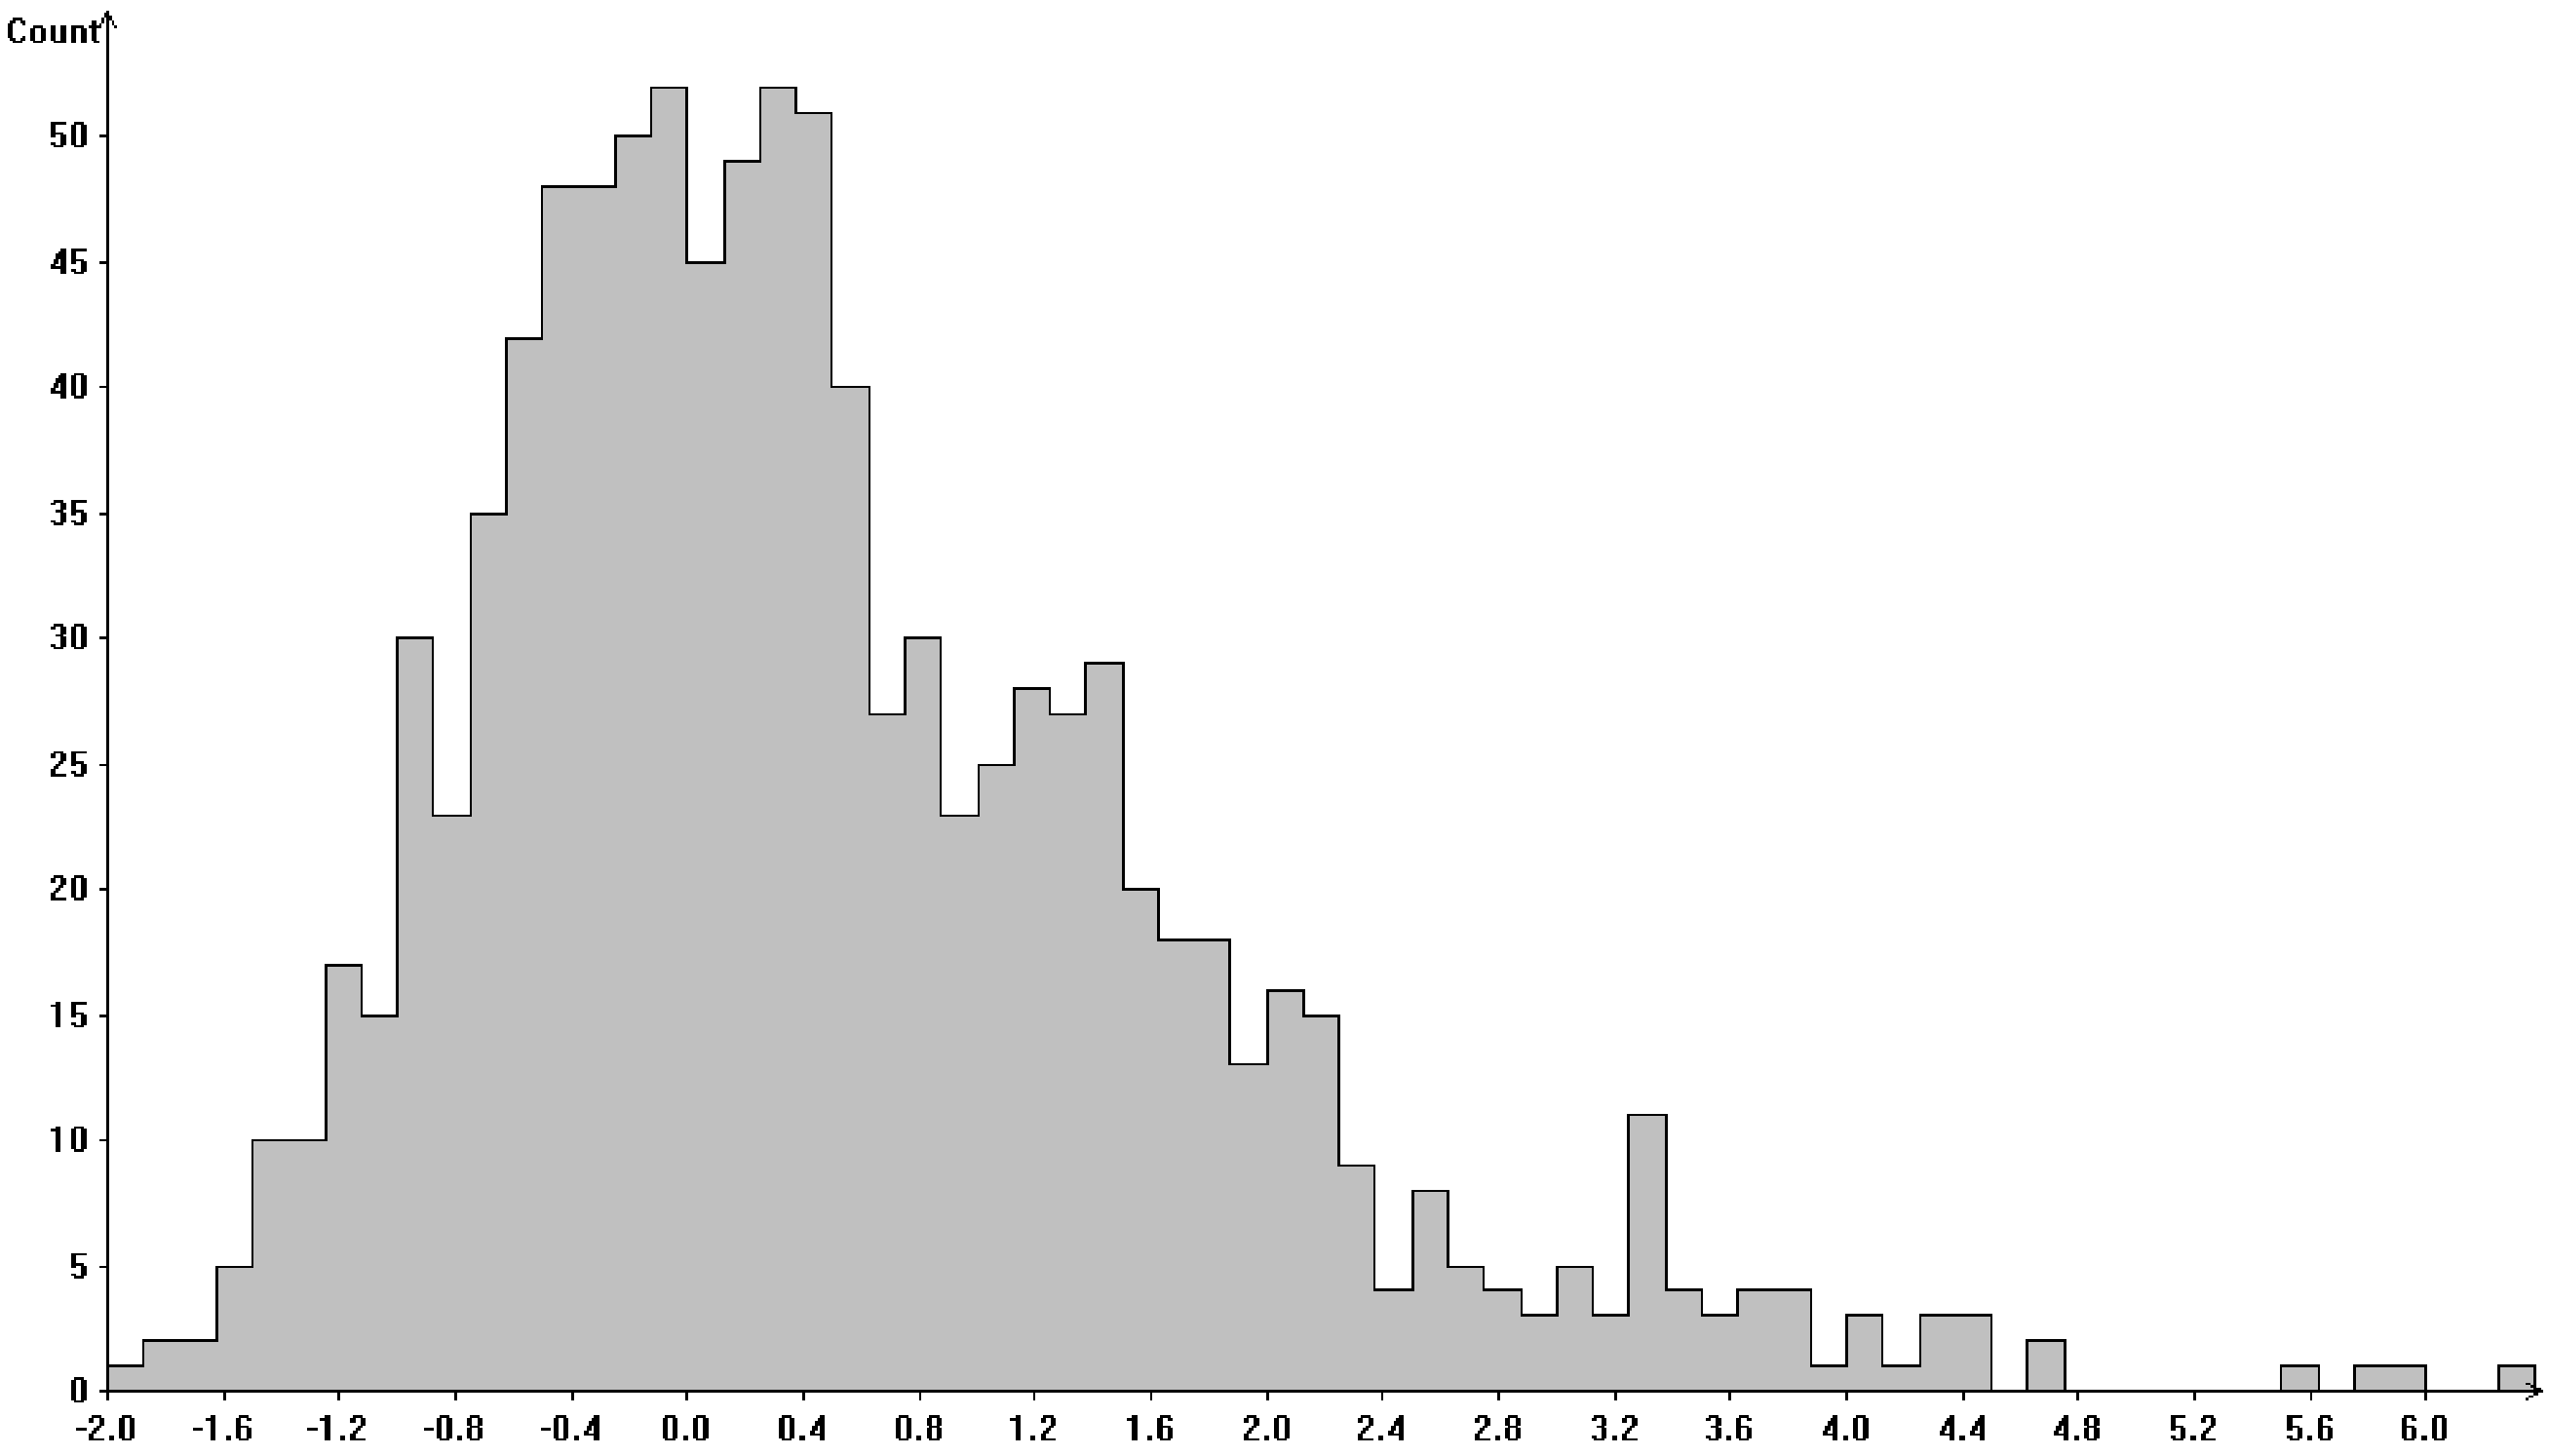
\includegraphics[width=12cm]{Figures/Histogram}
\caption{A typical histogram}\label{fig:histogram}
\end{figure}

A histogram is defined by three main parameters: $x_{\min}$, the
minimum of all values accumulated into the histogram, $w$, the bin
width and $n$, the number of bins. A bin is defined as an
interval. The $i\th$ bin of a histogram is the interval $\left[
x_{\min}+\left(i-1\right)w, x_{\min}+iw\right[$. The customary
convention is that the lower limit is included in the interval and
the higher limit excluded from the interval. The bin contents of a
histogram --- or histogram contents for short --- is the number of
times a value falls within each bin interval. Sometimes, a
histogram is defined by the minimum and maximum of the accumulated
values and the number of bins. The bin width is then computed as:
\begin{equation}
  w = {x_{\max} - x_{\min} \over n},
\end{equation}
where $x_{\max}$ is the maximum of the accumulated values.

In section \ref{sec:mlfhist} we shall need the error on the
contents of a histogram. In absence of any systematic
effects\footnote{A good example of systematic effect is when
values are computed from measurements made with an ADC. In this
case, the integer rounding of the ADC may interfere with the bin
sorting of the histogram.} the contents of each bin are
distributed according to a Poisson distribution. The standard
deviation of a Poisson distribution is the square root of the
average. The standard deviation is used as an estimator of the
error on the bin contents\footnote{This is not a contradiction to
what was said in section \ref{sec:moments}: the bin content is not
an average, but a counting}. If $n_i$ is the content of the $i\th$
bin of the histogram, the estimated error on the contents is
$\sqrt{n_i}$.

To obtain more information about the measured distribution, one
can also keep track of the number of values falling outside of the
histogram limits. The {\textsl underflow} of a histogram is defined as
the number of values falling below the minimum  of the accumulated
values. Similarly, the {\textsl overflow} of a histogram is defined as
the number of values falling on\footnote{This is different from
the definition of the underflow to be consistent with the fact
that the definition of a bin interval is open ended at the upper
limit.} or above the maximum of the accumulated values.

\subsection{Histograms --- General implementation}
\marginpar{Figure \ref{fig:statisticsclasses} with the box {\textbf
Histogram} grayed.} Our implementation of histogram also
accumulates the values into statistical moments. One can in
principle compute the statistical moments of the measured
distribution from the histogram contents. This determination,
however, depends strongly on the bin width, especially if the bin
width is large compared to the standard deviation. Thus, it is
preferable to use the original data when accumulating the
statistical moments. The net result is that a histogram has the
same polymorphic behavior as a statistical moment.

When defining a histogram, the histogram limits --- $x_{\min}$ and
$x_{\max}$ --- must be known in advance. This is not always
practical since it implies a first scan of the measurements to
determine the limits and a second scan to perform the accumulation
into the defined histogram. Thus, our implementation offers the
possibility of defining a histogram without predefined limits. In
this mode, the first values are cached into an array until a
sufficient number of data is available. When this happens, the
histogram limits are determined from the data and the cached
values are accumulated.

There are some cases when one would like to accumulates all the
values within the histogram limits. The proposed implementation
allows this by changing the histogram limits accordingly when a
new value falls outside of the current histogram limits. When a
histogram is accumulated in this mode the underflow and overflow
counts are always zero.

When the histogram limits are computed automatically, it can
happen that these limits have odd values. For example, if the
minimum value is 2.13456 and the maximum value is 5.1245,
selecting a number of bins of 50 would yield a bin width of
0.0597988. Of course such value for the bin width is quite
undesirable in practice. A similar thing can happen if the
application creating the histogram obtains the minimum and maximum
values from a computation or an automatic measuring device. To
avoid such silly parameters, our implementation computes a
reasonable limit and bin width by rounding the bin width to the
nearest reasonable scale at the order of magnitude\footnote{Let us
recall that the order of magnitude is the power of ten of a
number.} of the bin with. The possible scales are chosen to be
easily computed by a human. In our example, the order of magnitude
is $-2$. The bin width is then selected to be 0.075 and the
minimum and maximum are adjusted to be integral multiples of the
bin width enclosing the given limits. In our example, there are
$2.1$ and $5.175$ and the number of bins becomes 41 instead of 50.

\subsection{Histograms --- Smalltalk implementation}
\label{sec:shistogram} Listing \ref{ls:histogram} shows the
implementation of a histogram in Smalltalk. The following code
shows how to use the class {\texttt PMHistogram} to accumulate
measurements into a histogram.
\begin{displaycode}{Smalltalk}
 | histogram valueStream |
 histogram := PMHistogram new.
 [ valueStream atEnd ]
        whileFalse: [ histogram accumulate: valueStream next ].
\hfil {\texttt<\textsl printing or display of the histogram\texttt >}\hfil
\end{displaycode}

This example assumes that the measurement of the random variable
are obtained from a stream. The exact implementation of the stream
is not shown here.

After the declarative statements, the first executable statement
creates a new instance of the class {\texttt DhbHistogram} with the
default settings: automatic determination of the limits for 50
desired bins. The next two lines are the accumulation proper using
a {\texttt whileFalse:} construct and the general behavior of a
stream. This code is very similar to the code example presented in
section \ref{sec:smoments}. Extracting the parameters of the
distribution can also be performed from the histogram.

\noindent The next example shows how to declare a histogram with
given limits (2 and 7) and a desired number of bins of 50:
\begin{displaycode}{Smalltalk}
 | histogram valueStream |
 histogram := DhbHistogram new.
 histogram setRangeFrom: 2.0 to: 7.0 bins: 100.
\hfil {\texttt<\textsl the rest is identical to the previous example\texttt
>}\hfil
\end{displaycode}

\noindent The class {\texttt DhbHistogram} has the following instance
variables:
\begin{description}
  \item[\texttt minimum] the minimum of the accumulated values, that
  is $x_{\min}$,
  \item[\texttt binWidth] the bin width, that is $w$,
  \item[\texttt overflow] a counter to accumulate the overflow of the histogram,
  \item[\texttt underflow] a counter to accumulate the underflow of the histogram,
  \item[\texttt moments] an instance of the class {\texttt
  DhbFixedStatisticalMoments} to accumulate statistical moments up
  to the $4\th$ order (\cf section \ref{sec:srobustmoment}) with
  minimal rounding errors.
  \item[\texttt contents] the contents of the histogram, that is an
  array of integers,
  \item[\texttt freeExtent] a Boolean flag denoting whether the limits
  of the histogram can be adjusted to include all possible values,
  \item[\texttt cacheSize] the size of the cache allocated to collect
  values for an automatic determination of the histogram limits,
  \item[\texttt desiredNumberOfBins] the number of bins desired by the
  calling application.
\end{description}

Since there are many ways to declare a histogram, there is a
single creation method {\texttt new}, which calls in turn a single
standard initialization method {\texttt initialize}. In this mode. the
histogram is created with undefined limits --- that is, the first
accumulated values are cached until a sufficient number is
available for an automatic determination of the limits --- and a
default number of bins. The default number of bins is defined by
the class method {\texttt defaultNumberOfBins}.

\noindent Four methods allow to change the default initialization.

The method {\texttt setRangeFrom:to:bins:} allows the definition of
the parameters $x_{\min}$, $x_{\max}$ and $n$, respectively. The
method {\texttt setWidth:from:bins:} allows the definition of the
parameters $w$, $x_{\min}$ and $n$, respectively. In both cases,
the histogram limits and number of bins are adjusted to reasonable
values as explained at the end of section \ref{sec:histogram}.
These methods generate an error if the histogram is not cached, as
limits cannot be redefined while the histogram is accumulating.
The method {\texttt setDesiredNumberOfBins:} allows to overrule the
default number of bins. Finally, the method {\texttt freeExtent:}
takes a Boolean argument to define whether or not the limits must
be adjusted when an accumulated value falls outside of the
histogram limits. This method generates an error if any count has
been accumulated in the underflow or overflow.

The method {\texttt accumulate} is used to accumulate the values. If
the histogram is still cached --- that is when values are directly
accumulated into the cache for later determination of the limits
--- accumulation if delegated to the method {\texttt
accumulateInCache:}. In this mode, the instance variable {\texttt
contents} is an {\texttt OrderedCollection} collecting the values.
When the size of the collection is reaching the maximum size
allocated to the cache, limits are computed and the cache is
flushed. In direct accumulation mode, the bin index corresponding
to the value is computed. If the index is within the range, the
value is accumulated. Otherwise it is treated like an overflow or
an underflow. The method {\texttt processOverflows:for:} handles the
case where the accumulated values falls outside of the histogram
limits. If histogram limits cannot be adjusted it simply counts
the overflow or the underflow. Otherwise processing is delegated
to the methods {\texttt growsContents:}, {\texttt growsPositiveContents}
and {\texttt growsNegativeContents}, which adjust the histogram limits
according to the accumulated value.

The adjustment of the histogram limits to reasonable values is
performed by the method {\texttt adjustDimensionUpTo:}. This is made
when the limits are determined automatically. This method is also
used when the limits are specified using one of the initialization
methods.

There are many methods used to retrieve information from a
histogram. Enumerating them here would be too tedious. Method
names are explicit enough to get a rough idea of what each method
is doing; looking at the code should suffice for a detailed
understanding. The reader should just note that all methods
retrieving the parameters of the distribution, as discussed in
section \ref{sec:smoments}, are implemented by delegating the
method to the instance variable {\texttt moments}.

The iterator method {\texttt pointsAndErrorsDo:} is used for maximum
likelihood fit of a probability distribution. Smalltalk
implementation of maximum likelihood fit is discussed in section
\ref{sec:smlfhist}.

\begin{listing} Smalltalk implementation of histograms \label{ls:histogram}
$$\halign{ #\hfil&\quad#\hfil\cr {\sl Class}& {\Large\bf DhbHistogram}\cr
{\sl Subclass of }&{\tt Object}\cr\noalign{\vskip 1ex}

{\sl Instance variable names:}&\parbox[t]{4 in}{\tt  minimum binWidth overflow underflow moments contents freeExtent cacheSize desiredNumberOfBins }\cr\noalign{\vskip 1ex}}$$


Class methods
{\parskip 1ex\par\noindent}
{\bf defaultCacheSize}
\begin{verbatim}
    ^ 100
\end{verbatim}
{\bf defaultNumberOfBins}
\begin{verbatim}
    ^ 50
\end{verbatim}
{\bf integerScales}
\begin{verbatim}
   ^ self
\end{verbatim}

Instance methods
{\parskip 1ex\par\noindent}
{\bf accumulate:} {\tt aNumber}
\begin{verbatim}
    | bin |
    self isCached
        ifTrue: [ ^self accumulateInCache: aNumber ].
    bin := self binIndex: aNumber.
    ( bin between: 1 and: contents size)
        ifTrue: [ contents at: bin put: ( contents at: bin) + 1.
                     moments accumulate: aNumber.
                   ]
        ifFalse:[ self processOverflows: bin for: aNumber ].
\end{verbatim}
{\bf accumulateInCache:} {\tt aNumber}
\begin{verbatim}
    contents add: aNumber.
    contents size > cacheSize
        ifTrue: [ self flushCache ].
\end{verbatim}
{\bf adjustDimensionUpTo:} {\tt aNumber}
\begin{verbatim}
    | maximum |
    binWidth := self roundToScale: ( aNumber - minimum) / 
                                                  desiredNumberOfBins.
    minimum := ( minimum / binWidth) floor * binWidth.
    maximum := ( aNumber / binWidth) ceiling * binWidth.
    contents := Array new: ( ( maximum - minimum) / binWidth) 
                                                              ceiling.
    contents atAllPut: 0.
\end{verbatim}
{\bf average}
\begin{verbatim}
    ^ moments average
\end{verbatim}
{\bf binIndex:} {\tt aNumber}
\begin{verbatim}
    ^( ( aNumber - minimum) / binWidth) floor + 1
\end{verbatim}
{\bf binWidth}
\begin{verbatim}
    self isCached
        ifTrue: [ self flushCache].
    ^binWidth
\end{verbatim}
{\bf collectIntegralPoints:} {\tt aBlock}
\begin{verbatim}
    | answer bin lastContents integral norm x |
    self isCached
        ifTrue: [ self flushCache].
    answer := OrderedCollection new: ( contents size * 2 + 1).
    bin := self minimum.
    answer add: ( aBlock value: bin @ 0).
    integral := self underflow.
    norm := self totalCount.
    contents do:
        [ :each |
          integral := integral + each.
          x := integral / norm.
          answer add: ( aBlock value: bin @ x).
          bin := bin + binWidth.
          answer add: ( aBlock value: bin @ x).
        ].
    answer add: ( aBlock value: bin @ 0).
    ^ answer asArray
\end{verbatim}
{\bf collectPoints:} {\tt aBlock}
\begin{verbatim}
    | answer bin lastContents |
    self isCached
        ifTrue: [ self flushCache ].
    answer := OrderedCollection new: ( contents size * 2 + 1).
    bin := self minimum.
    answer add: (aBlock value: bin @ 0).
    contents do:
        [ :each |
          answer add: (aBlock value: bin @ each).
          bin := bin + binWidth.
          answer add: (aBlock value: bin @ each).
        ].
    answer add: (aBlock value: bin @ 0).
    ^ answer asArray
\end{verbatim}
{\bf count}
\begin{verbatim}
    ^ moments count
\end{verbatim}
{\bf countAt:} {\tt aNumber}
\begin{verbatim}
    | n |
    n := self binIndex: aNumber.
    ^ (n between: 1 and: contents size)
            ifTrue: [ contents at: n ]
            ifFalse: [ 0 ]
\end{verbatim}
{\bf countOverflows:} {\tt anInteger}
\begin{verbatim}
    anInteger > 0
        ifTrue: [ overflow := overflow + 1 ]
        ifFalse:[ underflow := underflow + 1 ].
\end{verbatim}
{\bf countsBetween:} {\tt aNumber1} {\bf and:} {\tt aNumber2}
\begin{verbatim}
    | n1 n2 answer |
    n1 := self binIndex: aNumber1.
    n2 := self binIndex: aNumber2.
    answer := ( contents at: n1) * ( ( binWidth * n1 + minimum) - 
                                                 aNumber1) / binWidth.
    n2 > contents size
        ifTrue: [ n2 := contents size + 1]
        ifFalse:[ answer := answer + ( ( contents at: n2) * ( 
      aNumber2 - ( binWidth * ( n2 - 1) + self maximum)) / binWidth)].
    ( n1 + 1) to: ( n2 - 1) do: [ :n | answer := answer + ( contents 
                                                              at: n)].
    ^ answer
\end{verbatim}
{\bf countsUpTo:} {\tt aNumber}
\begin{verbatim}
    | n answer |
    n := self binIndex: aNumber.
    n > contents size
        ifTrue: [ ^self count].
    answer := ( contents at: n) * ( aNumber - ( binWidth * ( n - 1) + 
                                            self minimum)) / binWidth.
    1 to: ( n - 1) do: [ :m | answer := answer + ( contents at: m)].
    ^ answer + underflow
\end{verbatim}
{\bf errorOnAverage}
\begin{verbatim}
    ^ moments errorOnAverage
\end{verbatim}
{\bf flushCache}
\begin{verbatim}
    | maximum values |
    minimum isNil
        ifTrue: [ minimum := contents isEmpty ifTrue: [ 0]
                                                                      
                                            ifFalse:[ contents first].
                   ].
    maximum := minimum.
    contents do:
        [ :each |
          each < minimum
            ifTrue: [ minimum := each]
            ifFalse:[ each > maximum
                            ifTrue: [ maximum := each].
                        ].
        ].
    maximum = minimum
        ifTrue: [ maximum := minimum + desiredNumberOfBins].
    values := contents.
    self adjustDimensionUpTo: maximum.
    values do: [ :each | self accumulate: each ].
\end{verbatim}
{\bf freeExtent:} {\tt aBoolean}
\begin{verbatim}
    ( underflow = 0 and: [ overflow = 0])
        ifFalse: [ self error: 'Histogram extent cannot be 
                                                          redefined'].
    freeExtent := aBoolean.
\end{verbatim}
{\bf growContents:} {\tt anInteger}
\begin{verbatim}
    anInteger > 0
        ifTrue: [ self growPositiveContents: anInteger ]
        ifFalse: [ self growNegativeContents: anInteger ].
\end{verbatim}
{\bf growNegativeContents:} {\tt anInteger}
\begin{verbatim}
    | n newSize newContents |
    n := 1 - anInteger.
    newSize := contents size + n.
    newContents := Array new: newSize.
    newContents
            at: 1 put: 1;
            replaceFrom: 2 to: n withObject: 0;
            replaceFrom: ( n + 1) to: newSize with: contents.
    contents := newContents.
    minimum := ( anInteger - 1) * binWidth + minimum.
\end{verbatim}
{\bf growPositiveContents:} {\tt anInteger}
\begin{verbatim}
    | n newContents |
    n := contents size.
    newContents := Array new: anInteger.
    newContents
            replaceFrom: 1 to: n with: contents;
            replaceFrom: ( n + 1) to: ( anInteger - 1) withObject: 0;
            at: anInteger put: 1.
    contents := newContents.
\end{verbatim}
{\bf initialize}
\begin{verbatim}
    freeExtent := false.
    cacheSize := self class defaultCacheSize.
    desiredNumberOfBins := self class defaultNumberOfBins.
    contents := OrderedCollection new: cacheSize.
    moments := DhbFixedStatisticalMoments new.
    overflow := 0.
    underflow := 0.
    ^ self
\end{verbatim}
{\bf inverseDistributionValue:} {\tt aNumber}
\begin{verbatim}
    | count x integral |
    count := self count * aNumber.
    x := self minimum.
    integral := 0.
    contents do:
        [ :each | | delta |
          delta := count - integral.
          each > delta
            ifTrue: [ ^self binWidth * delta / each + x].
          integral := integral + each.
          x := self binWidth + x.
        ].
    ^ self maximum
\end{verbatim}
{\bf isCached}
\begin{verbatim}
    ^ binWidth isNil
\end{verbatim}
{\bf isEmpty}
\begin{verbatim}
    ^ false
\end{verbatim}
{\bf kurtosis}
\begin{verbatim}
    ^ moments kurtosis
\end{verbatim}
{\bf lowBinLimitAt:} {\tt anInteger}
\begin{verbatim}
    ^ (anInteger - 1) * binWidth + minimum
\end{verbatim}
{\bf maximum}
\begin{verbatim}
    self isCached
        ifTrue: [ self flushCache ].
    ^ contents size * binWidth + minimum
\end{verbatim}
{\bf maximumCount}
\begin{verbatim}
    self isCached
        ifTrue: [ self flushCache ].
    ^contents inject: ( contents isEmpty ifTrue: [ 1] ifFalse:[ 
                                                      contents at: 1])
                    into: [ :max :each | max max: each]
\end{verbatim}
{\bf minimum}
\begin{verbatim}
    self isCached
        ifTrue: [ self flushCache ].
    ^ minimum
\end{verbatim}
{\bf overflow}
\begin{verbatim}
    ^ overflow
\end{verbatim}
{\bf processOverflows:} {\tt anInteger} {\bf for:} {\tt aNumber}
\begin{verbatim}
    freeExtent
        ifTrue: [ self growContents: anInteger.
                     moments accumulate: aNumber
                   ]
        ifFalse:[ self countOverflows: anInteger ].
\end{verbatim}
{\bf setDesiredNumberOfBins:} {\tt anInteger}
\begin{verbatim}
    anInteger > 0
        ifFalse:[ self error: 'Desired number of bins must be 
                                                           positive'].
    desiredNumberOfBins := anInteger.
\end{verbatim}
{\bf setRangeFrom:} {\tt aNumber1} {\bf to:} {\tt aNumber2} {\bf bins:} {\tt anInteger}
\begin{verbatim}
    self isCached
        ifFalse: [ self error: 'Histogram limits cannot be 
                                                          redefined'].
    minimum := aNumber1.
    self setDesiredNumberOfBins: anInteger;
           adjustDimensionUpTo: aNumber2.
\end{verbatim}
{\bf setWidth:} {\tt aNumber1} {\bf from:} {\tt aNumber2} {\bf bins:} {\tt anInteger}
\begin{verbatim}
    self isCached
        ifFalse: [ self error: 'Histogram limits cannot be 
                                                          redefined'].
    minimum := aNumber2.
    self setDesiredNumberOfBins: anInteger;
           adjustDimensionUpTo: ( aNumber1 * anInteger + aNumber2).
\end{verbatim}
{\bf skewness}
\begin{verbatim}
    ^ moments skewness
\end{verbatim}
{\bf standardDeviation}
\begin{verbatim}
    ^ moments standardDeviation
\end{verbatim}
{\bf totalCount}
\begin{verbatim}
    ^ moments count + underflow + overflow
\end{verbatim}
{\bf underflow}
\begin{verbatim}
    ^ underflow
\end{verbatim}
{\bf variance}
\begin{verbatim}
    ^ moments variance
\end{verbatim}


\end{listing}


\section{Random number generator}
\label{sec:random} When studying statistical processes on a
computer one often has to simulate the behavior of a random
variable\footnote{Another wide use for random number generators
are games.}. As we shall see in section \ref{sec:probdistr} it
suffice to implement a random generator for a uniform
distribution, that is a random variable whose probability density
function is constant over a given interval. Once such an
implementation is available, any probability distribution can be
simulated.

\rubrique{Linear congruential random generators} The most widely
used random number generators are linear congruential random
generators. Random numbers are obtained from the following series
\cite{Knuth2}:
\begin{equation}
\label{eq:crg}
  X_{n+1} = \left(aX_n+c\right) \mod m,
\end{equation}
where $m$ is called the modulus, $a$ the multiplier and $c$ the
increment. By definition, we have $0\leq X_n<m$ for all $n$. The
numbers $X_n$ are actually pseudo-random numbers since, for a
given modulus, multiplier and increment, the sequence of numbers
$X_1,\ldots,X_n$ is fully determined by the value $X_0$. The value
$X_0$ is called the seed of the series. In spite of its
reproducibility the generated series behaves very close to that of
random variable uniformly distributed between 0 and $m-1$. Then
the following variable:
\begin{equation}
  x_n = {X_n \over m},
\end{equation}
is a random rational number uniformly distributed between 0 and 1,
1 excluded.

In practice, the modulus, multiplier and increment must be chosen
quite carefully to achieve a good randomness of the series. Don
Knuth \cite{Knuth2} gives a series of criteria for choosing the
parameters of the random number generator. If the parameters are
correctly chosen, the seed $X_0$ can be assigned to any value.

\rubrique{Additive sequence generators} Another class of random
generators are additive sequence generators \cite{Knuth2}. The
series of pseudo-random numbers is generated as follows:
\begin{equation}
  X_n = \left(X_{n-l}+X_{n-k}\right) \mod m,
\end{equation}
where $m$ is the modulus as before and $l$ and $k$ are two indices
such that $l<k$. These indices must be selected carefully.
\cite{Knuth2} contains a table of suitable indices. The initial
series of numbers $X_1,\ldots,X_k$ can be any integers not all
even.

Generators based on additive sequences are ideal to generate
floating point numbers. If this case, the modulo operation on the
modulus is not needed. Instead, one simply checks whether or not
the newly generated number is larger than 1. Thus, the series
becomes:
\begin{equation}
\label{eq:addseqrandom}
  \begin{array}{lcl}
  y_n&=&x_{n-l}+x_{n-k},\\*[2ex]
  x_n&=&\left\{
    \begin{array}{ll}
    y_n&\mbox{\quad if $y_n<1$,}\\
    y_n-1&\mbox{\quad if $y_n\geq 1$,}\\
    \end{array}
  \right.
  \end{array}
\end{equation}
It is clear that the evaluation above is much faster than that of
equation \ref{eq:crg}. In practice, the additive sequence
generator is about 4 times faster. In addition, the length of the
sequence is larger than that of a  congruential random generator
with the same modulus.

In our implementation we have selected the pair of numbers
$\left(24,55\right)$ corresponding to the generator initially
discovered by G.J. Mitchell and D.P. Moore\cite{Knuth2}. The
corresponding sequence has a length of $2^{55}-1$. In our tests
(\cf below) we have found that the randomness of this generator is
at least as good as that of the congruential random generator. The
initial series $x_1,\ldots,x_{55}$ is obtained from the
congruential random generator.

In \cite{Knuth2} Don Knuth describes a wealth of test to
investigate the randomness of random number generators. Some of
these tests are also discussed in \cite{LawKel}. To study the
goodness of our proposed random generators, we have performed two
types of tests: a $\chi^2$ test and a correlation test.

The $\chi^2$ test is performed on a histogram, in which values
generated according to a probability distributions have been
accumulated. Then, a $\chi^2$ confidence level (\cf section
\ref{sec:chitest}) is calculated against the theoretical curve
computed using the histogram bin width, the number of generated
values and the parameters of the distribution. A confidence level
should be larger than $60\%$ indicates that the probability
distribution is correctly generated. When using distributions
requiring the generation of several random numbers to obtain one
value --- Normal distribution (2 values), gamma distribution (2
values) and beta distribution (4 values)
--- one can get a good confidence that short term
correlations\footnote{Pseudo random number generators have a
tendency to exhibit correlations in the series. That is, the
number $X_n$ can be correlated to the number $X_{n-k}$ for each
$n$ and a given $k$.} are not creating problems. The code for this
test is given in the code examples \ref{exs:chitest}. In this test the Mitchell-Moore
generator gives results similar to that of the congruential random
generator.

The correlation test is performed by computing the covariance
matrix (\cf section \ref{sec:covmatrix}) of vectors of given
dimension (between 5 and 10). The covariance matrix should be a
diagonal matrix with all diagonal elements equal to $1/12$, the
variance of a uniform distribution. Deviation from this
theoretical case should be small. Here longer correlations can be
investigated by varying the dimension of the generated vectors. In
this test too, the Mitchell-Moore generator gives results similar
to that of the congruential random generator.

\rubrique{Bit-pattern generators} The generators described above
are suitable to the generation of random values, but not for the
generation of random bit patterns \cite{Knuth2}, \cite{Press}. The
generation of random bit patterns can be achieved with generator
polynomials. Such polynomials are used in error correction codes
for their abilities to produce sequences of numbers with a maximum
number of different bits. For example the following polynomial
\begin{equation}
\label{eq:ranpolgen}
  G\left(x\right) = x^{16} + x^{12} +x^5 + 1,
\end{equation}
is a good generator for random patterns of 16 bits\footnote{\cf O.
Yamada, K. Yamazaki and D.H.Besset, {\em An Error-Correction
Scheme for an Optical Memory Card System}, 1990 International
Symposium on Information Theory and its Applications (ISITA'90),
Hawaii, USA, November 27-30, 1990.}. Of course, the evaluation of
equation \ref{eq:ranpolgen} does not require the computation of
the polynomial. The following algorithm can be used: {\parskip 0pt
\begin{enumerate}
  \item Set $X_{n+1}$ to $X_n$ shifted by one position to the left
  and truncated to 16 bits ($X_{n+1}=2X_n \mod 2^{16}$),
  \item If bit 15 (least significant bit being 0) of $X_n$ is set,
  set $X_{n+1}$ to the bit wise exclusive OR of $X_{n+1}$ with
  {\texttt 0x1021}.
\end{enumerate}}
\noindent Other polynomials are given in \cite{Press}.

Random bit patterns are usually used to simulate hardware
behavior. They are rarely used in statistical analysis. A concrete
implementation of a random bit pattern generator is left as an
exercise to the reader.

\subsection{Random number generator --- Smalltalk implementation}
\marginpar{Figure \ref{fig:statisticsclasses} with the boxes {\textbf
CongruentialRandomNumberGenerator} and {\textbf
MitchellMooreGenerator} grayed.} Listing \ref{ls:randomcong} shows
the implementation of a congruential random generator in
Smalltalk. Listing \ref{ls:randomseq} shows the implementation of
a additive sequence random generator in Smalltalk. Listing
\ref{ls:randomuse} shows usage of the generator for standard use.

\noindent The class {\texttt DhbCongruentialRandomNumberGenerator} has
three public methods:
\begin{description}
  \item[\texttt value] returns the next random number of the series,
  that is $X_n$, a number between $0$ and $m$,
  \item[\texttt floatValue] returns the next random floating number,
  that is the value $X_n / m$,
  \item[\texttt integerValue:] returns a random integer, whose values
  are between 0 and the specified argument.
\end{description}
When calling any of the above methods, the next random number of
the series is obtained using equation \ref{eq:crg}.

There are several ways of using a random number generator. If
there is no specific requirement the easiest approach is to use
the instance provided by default creation method ({\texttt new})
returning a \patstyle{singleton}. The next example shows how to
proceed assuming the application uses the values generated by the
random generator directly:
\begin{displaycode}{Smalltalk}
 | generator x |
 generator := DhbCongruentialRandomNumberGenerator new.
\hfil{\texttt <\textsl Here is where the generator is used\texttt
>}\hfil

 x := generator value.
\end{displaycode}

If one needs several series which must be separately reproducible,
one can assign several generators, one for each series. The
application can use predefined numbers for the seed of each
series. Here is a complete example assuming that the generated
numbers must be floating numbers.
\begin{displaycode}{Smalltalk}

 | generators seeds index x |

 {\texttt seeds := <\textsl an array containing the desired seeds\texttt >}

 generators := seeds collect:
           [ :each | DhbCongruentialRandomNumberGenerator seed: each].

\noindent\hskip 5ex{\texttt <\textsl Here is where the various generators
are used\texttt
>}\hfil \\
\hskip 5ex{\texttt <index \textsl is the index of the desired series\texttt
>}\hfil

 x := ( generators at: index) floatValue.
\end{displaycode}

In game applications, it is of course not desirable to have a
reproducible series. In this case, the easiest way is to use the
time in milliseconds as the seed of the series. This initial value
is sufficiently hard to reproduce to give the illusion of
randomness. Furthermore the randomness of the series guarantees
that two series generated at almost the same time are quite
different. Here is how to do it.
\begin{displaycode}{Smalltalk}

 | generator x |
 generator := DhbCongruentialRandomNumberGenerator
                        seed: Time millisecondClockValue.

\hfil{\texttt <\textsl Here is where the generator is used\texttt
>}\hfil

 x := (generator integerValue: 20) + 1.
\end{displaycode}

In this last example, the generated numbers are integers between 1
and 20.

\rubrique{Implementation} The class {\texttt
DhbCongruentialRandomNumberGenerator} has the following instance
variables:
\begin{description}
  \item[\texttt constant] the increment $c$,
  \item[\texttt modulus] the modulus $m$,
  \item[\texttt multiplicator] the multiplier $a$ and
  \item[\texttt seed] the last generated number $X_{n-1}$.
\end{description}
There are three instance creation methods. The method {\texttt new}
returns a \patstyle{singleton} instance containing parameters from
\cite{Knuth2}. The method {\texttt seed:} allows one to create an
instance to generate a series of random number starting at a given
seed. Finally the method {\texttt constant:multiplicator:modulus:}
creates a congruential random number generator based on supplied
parameters. Readers tempted to use this method are strongly
advised to read \cite{Knuth2} and the references therein
thoroughly. Then, they should perform tests to verify that their
parameters are indeed producing a series with acceptable
randomness.

The modulus of the standard parameters has 32 bits. In the
Smalltalk implementation, however, the evaluation of equation
\ref{eq:crg} generates integers larger than 32 bits. As a result,
the generation of the random numbers is somewhat slow, as it is
using multiple precision integers. Using floating
number\footnote{The author is grateful to Dave N. Smith of IBM for
this useful tip.} does not disturb the evaluation of equation
\ref{eq:crg} and is significantly faster since floating point
evaluation is performed on the hardware. The generation of random
numbers using floating point parameters is about 3 times faster
than with integer parameters. This can easily be verified by the
reader.

\begin{listing} Smalltalk implementation of congruential random number generators
\label{ls:randomcong}
$$\halign{ #\hfil&\quad#\hfil\cr {\sl Class}& {\Large\bf DhbCongruentialRandomNumberGenerator}\cr
{\sl Subclass of }&{\tt Object}\cr\noalign{\vskip 1ex}

{\sl Instance variable names:}&\parbox[t]{4 in}{\tt  constant modulus multiplicator seed }\cr\noalign{\vskip 1ex}
{\sl Class variable names:}&\parbox[t]{4 in}{\tt  UniqueInstance }\cr\noalign{\vskip 1ex}}$$


Class methods
{\parskip 1ex\par\noindent}
{\bf constant:} {\tt aNumber1} {\bf multiplicator:} {\tt aNumber2} {\bf modulus:} {\tt aNumber3}
\begin{verbatim}
    ^ super new 
        initialize: aNumber1
        multiplicator: aNumber2
        modulus: aNumber3

\end{verbatim}
{\bf new}
\begin{verbatim}
    UniqueInstance isNil
        ifTrue: [ UniqueInstance := super new initialize.
                     UniqueInstance setSeed: 1 ].
    ^ UniqueInstance
\end{verbatim}
{\bf seed:} {\tt aNumber}
\begin{verbatim}
    ^ super new initialize; setSeed: aNumber; yourself
\end{verbatim}

Instance methods
{\parskip 1ex\par\noindent}
{\bf floatValue}
\begin{verbatim}
    ^ self value asFloat / modulus
\end{verbatim}
{\bf initialize}
\begin{verbatim}
    self initialize: 2718281829.0 multiplicator: 3141592653.0 
                                                modulus: 4294967296.0.
\end{verbatim}
{\bf initialize:} {\tt aNumber1} {\bf multiplicator:} {\tt aNumber2} {\bf modulus:} {\tt aNumber3}
\begin{verbatim}
    constant := aNumber1.
    modulus := aNumber2.
    multiplicator := aNumber3.
    self setSeed: 1.
\end{verbatim}
{\bf integerValue:} {\tt anInteger}
\begin{verbatim}
    ^ (self value \\ ( anInteger * 1000)) // 1000
\end{verbatim}
{\bf setSeed:} {\tt aNumber}
\begin{verbatim}
    seed := aNumber.
\end{verbatim}
{\bf value}
\begin{verbatim}
    seed := (seed * multiplicator + constant) \\ modulus.
    ^ seed
\end{verbatim}


\end{listing}

\noindent The class {\texttt DhbMitchellMooreGenerator} implements a
random number generator with additive sequence. It has two public
methods:
\begin{description}
  \item[\texttt floatValue] returns the next random floating number,
  that is the value $x_n$,
  \item[\texttt integerValue:] returns a random integer, whose values
  are between 0 and the specified argument.
\end{description}
When calling any of the above methods, the next random number of
the series is obtained using equation \ref{eq:addseqrandom}. The
series of generated numbers are all floating points.

The creation methods {\texttt new} and {\texttt seed:} are used exactly as
the corresponding methods of the class {\texttt
DhbCongruentialRandomNumberGenerator}. Please refer to the code
examples \ref{codex:crgdefault} and \ref{codex:crgseeded}. Both
methods use the congruential random number generator to generate
the initial series of numbers $x_1,\ldots,x_{55}$. The class
method {\texttt constants:lowIndex:} offers a way to define the
numbers $k$ and $l$ as well as the initial series of numbers. The
reader wishing to use this method should consult the table of {\textsl
good} indices $k$ and $l$ in \cite{Knuth2}.

\begin{listing} Smalltalk implementation of an additive sequence random number generator
\label{ls:randomseq}
$$\halign{ #\hfil&\quad#\hfil\cr {\sl Class}& {\Large\bf DhbMitchellMooreGenerator}\cr
{\sl Subclass of }&{\tt Object}\cr\noalign{\vskip 1ex}

{\sl Instance variable names:}&\parbox[t]{4 in}{\tt  randoms lowIndex highIndex }\cr\noalign{\vskip 1ex}
{\sl Class variable names:}&\parbox[t]{4 in}{\tt  UniqueInstance }\cr\noalign{\vskip 1ex}}$$


Class methods
{\parskip 1ex\par\noindent}
{\bf constants:} {\tt anArray} {\bf lowIndex:} {\tt anInteger}
\begin{verbatim}
    ^super new initialize: anArray lowIndex: anInteger

\end{verbatim}
{\bf default}
\begin{verbatim}
    | congruentialGenerator |
    congruentialGenerator := DhbCongruentialRandomNumberGenerator 
                                                                  new.
    ^ self generateSeeds: congruentialGenerator
\end{verbatim}
{\bf generateSeeds:} {\tt congruentialGenerator}
\begin{verbatim}

\end{verbatim}
{\bf new}
\begin{verbatim}
    UniqueInstance isNil
        ifTrue: [ UniqueInstance := self default].
    ^ UniqueInstance
\end{verbatim}
{\bf seed:} {\tt anInteger}
\begin{verbatim}
    | congruentialGenerator |
    congruentialGenerator := DhbCongruentialRandomNumberGenerator 
                                                      seed: anInteger.
    ^self generateSeeds: congruentialGenerator
\end{verbatim}

Instance methods
{\parskip 1ex\par\noindent}
{\bf floatValue}
\begin{verbatim}
    | x |
    x := (randoms at: lowIndex) + (randoms at: highIndex).
    x < 1.0 ifFalse: [x := x - 1.0].
    randoms at: highIndex put: x.
    highIndex := highIndex + 1.
    highIndex > randoms size ifTrue: [highIndex := 1].
    lowIndex := lowIndex + 1.
    lowIndex > randoms size ifTrue: [lowIndex := 1].
    ^ x

\end{verbatim}
{\bf initialize:} {\tt anArray} {\bf lowIndex:} {\tt anInteger}
\begin{verbatim}
    randoms := anArray.
    lowIndex := anInteger.
    highIndex := randoms size.
    ^ self
\end{verbatim}
{\bf integerValue:} {\tt anInteger}
\begin{verbatim}
    ^ (self floatValue * anInteger) truncated
\end{verbatim}


\end{listing}

For simple simulation, one wishes to generate a random number ---
floating or integer --- within certain limits. Here are
convenience methods implemented for the class {\texttt Number} and
{\texttt Integer}. These methods frees the user from keeping track of
the instance of the random number generator. For example, the
following Smalltalk expression
\begin{quote}
\begin{verbatim}
 50 random
\end{verbatim}
\end{quote}
\noindent generates an integer random number between 0 and 49
included. Similarly the following Smalltalk expression
\begin{quote}
\begin{verbatim}
 2.45 random
\end{verbatim}
\end{quote}
\noindent generates a floating random number between 0 and $2.45$
excluded. Finally the following Smalltalk expression
\begin{quote}
\begin{verbatim}
 Number random
\end{verbatim}
\end{quote}
\noindent generates a floating random number between 0 and 1
excluded.
\begin{listing} Smalltalk implementation of random number generators
\label{ls:randomuse}
$$\halign{ #\hfil&\quad#\hfil\cr {\sl Class}& {\Large\bf Integer}\cr
{\sl Subclass of }&{\tt Number}\cr\noalign{\vskip 1ex}
}$$


Instance methods
{\parskip 1ex\par\noindent}
{\bf random}
\begin{verbatim}
    ^DhbMitchellMooreGenerator new integerValue: self
\end{verbatim}


$$\halign{ #\hfil&\quad#\hfil\cr {\sl Class}& {\Large\bf Number}\cr
{\sl Subclass of }&{\tt Magnitude}\cr\noalign{\vskip 1ex}
}$$


Class methods
{\parskip 1ex\par\noindent}
{\bf random}
\begin{verbatim}
    ^ DhbMitchellMooreGenerator new floatValue
\end{verbatim}



Instance methods
{\parskip 1ex\par\noindent}
{\bf random}
\begin{verbatim}
    ^ self class random * self
\end{verbatim}


\end{listing}

\section{Probability distributions}
\label{sec:probdistr}A probability density function defines the
probability of finding a continuous random variable within an
infinitesimal interval. More precisely, the probability density
function $P\left(x\right)$ gives the probability for a random
variable to take a value lying in the interval
$\left[x,x+dx\right[$. A probability density function is a special
case of a one variable function described in section
\ref{sec:function}.

The moment of $k^{\mathop{\textrm th}}$ order for a probability
density function $P\left(x\right)$ is defined by:
\begin{equation}
\label{eq:probdensity}
  M_k=\int x^k P\left(x\right) dx,
\end{equation}
where the range of the integral is taken over the range where the
function $P\left(x\right)$ is defined. By definition probability
density functions are normalized, that is, $M_0$ is equal to 1.

As for statistical moments, one defines the mean or average of the
distribution as:
\begin{equation}
  \mu=M_1=\int x P\left(x\right) dx.
\end{equation}
Then the central moment of $k^{\mathop{\textrm th}}$ order is defined
by:
\begin{equation}
  m_k=\int \left(x-\mu\right)^k P\left(x\right) dx.
\end{equation}
In particular the variance is defined as $m_2$, the central moment
of second order. The standard deviation, $\sigma$, is the square
root of $m_2$. The skewness and kurtosis\footnote{In old
references the kurtosis, as defined here, is called excess; then,
the kurtosis is defined as the square of the excess;
\cite{AbrSteg} \eg.} of a probability density function are
respectively defined as:
\begin{equation}
  \omega={\displaystyle m_3 \over\displaystyle {\root 3/2 \of m_2}}
  ={\displaystyle m_3 \over\displaystyle \sigma^3}\mbox{\quad and}
\end{equation}
\begin{equation}
  \kappa={\displaystyle m_4 \over\displaystyle m_2^2}-3
  ={\displaystyle m_4 \over\displaystyle \sigma^4}-3.
\end{equation}

The distribution function, also called acceptance function or
repartition function, is defined as the probability for the random
variable to have a value smaller or equal to a given value. For a
probability density function defined over all real numbers we
have:
\begin{equation}
\label{eq:defdistr}
  F\left(t\right)=\prob\left(x<t\right)=\int_{-\infty}^t P\left(x\right)
  dx.
\end{equation}
If the probability density function $P\left(x\right)$ is defined
over a restricted range, the lower limit of the integral in
equation \ref{eq:defdistr} must be changed accordingly. For
example, if the probability density function is defined for $x\geq
x_{\min}$ , the distribution function is given by:
\begin{equation}
\label{eq:defdistrmin}
  F\left(t\right)=\prob\left(x<t\right)=\int_{x_{\min}}^t P\left(x\right)
  dx.
\end{equation}
Instead of the distribution function,  the name centile is
sometimes used to refer to the value of the distribution function
expressed in percent. This kind of terminology is frequently used
in medical and natural science publications. For example, a value
$x$ is said to be at the $10^{\mathop{\textrm th}}$ centile if
$F\left(t\right)=1/10$; in other words, there is a ten-percent
chance of observing a value less than or equal to $t$\footnote{A
centile can also be quoted for a value relative to a set of
observed values.}.

The interval acceptance function measures the probability for the
random variable to have a value between two given values. That is
\begin{equation}
\label{eq:defacceptint}
  F\left(x_1,x_2\right)=\prob\left(x_1\le x<x_2\right)
  =\int_{x_1}^{x_2} P\left(x\right)dx,
\end{equation}
\begin{equation}
\label{eq:defacceptdiff}
  F\left(x_1,x_2\right)=F\left(x_2\right)-F\left(x_1\right).
\end{equation}
If the integral of equation \ref{eq:defdistr} can be resolved into
a closed expression or if it has a numerical approximation, the
evaluation of the interval acceptance function is made using
equation \ref{eq:defacceptdiff}. Otherwise the interval acceptance
function must be evaluated using Romberg integration (\cf section
\ref{sec:romberg}) applied to equation \ref{eq:defacceptint}.

The inverse of the repartition function is frequently used. For
example, in order to determine an acceptance threshold in a
decision process, one needs to determine the variable $t$ such
that the repartition function is equal to a given value $p$. In
other words, $t=F^{-1}\left(p\right)$. For example, the threshold
of a coin detection mechanism to only reject $99.9\%$ of the good
coins is $F^{-1}\left(0.999\right)$. If the distribution function
is not invertible, one can solve this equation using the Newton's
zero-finding method exposed in section \ref{sec:snewton}. Newton's
zero-finding method is especially handy since the derivative of
the function is known: it is the probability density function.
Since $F\left(x\right)$ is strictly monotonous between 0 and 1 a
unique solution is guaranteed for any $p$ within the open interval
$\left]0,1\right[$. The initial value for the search can be
obtained from Markov's inequality \cite{CorLeiRiv}, which can be
written in the form:
\begin{equation}
  t\le {\displaystyle \mu \over\displaystyle 1-F\left(t\right)}
\end{equation}
If no closed expression exists for the distribution function (it
is determined using numerical integration \eg) the computation of
the inverse value is best obtained by interpolating the inverse
function over a set of by tabulated values (\cf section
\ref{ch:interpolation}).

The inverse of the distribution function is also used to generate
a random variable distributed according to the distribution.
Namely, if $r$ is a random variable uniformly distributed between
0 and 1, then the variable $x=F^{-1}\left(r\right)$ is a random
variable distributed according to the distribution whose
distribution function is $F\left(x\right)$. In practice this
method can only be used if a closed expression exists for the
distribution function, otherwise the function must be tabulated
and Newton interpolation can be used on the inverse function (\cf
section \ref{sec:newtoninterpol}). For most known distributions,
however, special algorithms exist to generate random values
distributed according to a given distribution. Such algorithms are
described in \cite{LawKel}. They are not discussed here, but the
code is included in each implementation of the specific
probability distribution.

In the rest of this chapter we shall present the distributions
used in this book. Other important distributions are presented in
appendix \ref{ch:distributions}.

\subsection{Probability distributions --- Smalltalk implementation}
\marginpar{Figure \ref{fig:statisticsclasses} with the boxes {\textbf
ProbabilityDensity} and {\textbf
ProbabilityDensityWithUnknownDistribution} grayed.} Table
\ref{tb:distrgenimpl} shows the description of the public methods
of the implementation.
\begin{table}[h]
  \centering
  \caption{Public methods for probability density functions}
  \label{tb:distrgenimpl}
\vspace{1 ex}
\begin{tabular}{|l | l |} \hline
  Description & \hfil Smalltalk \\ \hline
  $P\left(x\right)$ & {\texttt value:} \\
  $F\left(x\right)$ & {\texttt distributionValue:} \\
  $F\left(x_1,x_2\right)$ & {\texttt acceptanceBetween:and:} \\
  $F^{-1}\left(x\right)$ & {\texttt inverseDistributionValue:} \\
  $x^{\dag}$ & {\texttt random} \\
  \hline
  $\bar{x}$ & {\texttt average} \\
  $\sigma^2$ & {\texttt variance} \\
  $\sigma$ & {\texttt standardDeviation} \\
  skewness & {\texttt skewness} \\
  kurtosis & {\texttt kurtosis} \\
  \hline
\end{tabular}
$\dag$ $x$ represents the random variable itself. In other words,
the method {\texttt random} returns a random value distributed
according to the distribution.
\end{table}

Depending on the distribution, closed expressions for the variance
or the standard deviation exist. Here general methods are supplied
to compute one from the other. Subclasses must implement at least
one of them; otherwise a stack overflow will result.

Methods to compute skewness and kurtosis are supplied, but return
{\texttt nil} in Smalltalk. A very general
implementation could have used explicit integration. The
integration interval, however, maybe infinite and a general
integration strategy cannot easily be supplied. Subclasses are
expected to implement both methods.

As we have quoted earlier a probability density function is a
function, as defined in section \ref{sec:function}. Since the
distribution function is also a function, a \patstyle{Adapter}
must be provided to create a function (as defined in section
\ref{sec:function}) for the distribution function.

Listing \ref{ls:probdistr} shows the implementation of a general
probability density distribution in Smalltalk. The class {\texttt
DhbProbabilityDensity} is an abstract implementation. Concrete
implementation of probability density distributions are subclass
of it.

The method {\texttt distributionValue:} returning the value of the
distribution function must be implemented by the subclass. The
method to compute the interval acceptance functions is using
equation \ref{eq:defacceptdiff} .

The inverse acceptance function is defined with two methods, one
public and one private. The public method verifies the range of
the argument, which must lie between 0 and 1. The private method
uses the class {\texttt DhbNewtonZeroFinder} discussed in section
\ref{sec:snewton}. The derivative needed by the Newton zero finder
is the probability density function itself since, by definition,
it is the derivative of the acceptance function (\cf equation
\ref{eq:defdistr}).

Finally the class creation method {\texttt fromHistogram:} creates a
new instance of a probability distribution with parameters derived
using a quick approximation from the data accumulated into the
supplied histogram; the derivation assumes that the accumulated
data are distributed according to the distribution. This method is
used to compute suitable starting values for least square or
maximum likelihood fits (\cf chapter \ref{ch:estimation}). The
convention is that this methods returns {\texttt nil} if the
parameters cannot be obtained. Thus, returning {\texttt nil} is the
default behavior for the superclass since this method is specific
to each distribution. The estimation of the parameters is usually
made using the statistical moments of the histogram and comparing
them to the analytical expression of the distribution's parameter.

\begin{listing} Smalltalk implementation of a probability distribution
\label{ls:probdistr}
$$\halign{ #\hfil&\quad#\hfil\cr {\sl Class}& {\Large\bf DhbProbabilityDensity}\cr
{\sl Subclass of }&{\tt Object}\cr\noalign{\vskip 1ex}
}$$


Class methods
{\parskip 1ex\par\noindent}
{\bf distributionName}
\begin{verbatim}
    ^ 'Unknown distribution'
\end{verbatim}
{\bf fromHistogram:} {\tt aHistogram}
\begin{verbatim}
    ^ nil
\end{verbatim}

Instance methods
{\parskip 1ex\par\noindent}
{\bf acceptanceBetween:} {\tt aNumber1} {\bf and:} {\tt aNumber2}
\begin{verbatim}
    ^ (self distributionValue: aNumber2) - (self distributionValue: 
                                                             aNumber1)
\end{verbatim}
{\bf approximatedValueAndGradient:} {\tt aNumber}
\begin{verbatim}
    | delta parameters dp gradient n |
    parameters := self parameters.
    n := parameters size.
    dp := self value: aNumber.
    delta := Array new: n.
    delta atAllPut: 0.
    gradient := DhbVector new: n.
    1 to: n do:
        [ :k |
          delta at: k put: ( parameters at: k) * 0.0001.
          self changeParametersBy: delta.
          gradient at: k put: ( ( ( self value: aNumber) - dp) / ( 
                                                        delta at: k)).
          delta at: k put: ( delta at: k ) negated.
          k > 1
            ifTrue: [ delta at: ( k - 1) put: 0].
        ].
    self changeParametersBy: delta.
    ^Array with: dp with: gradient
\end{verbatim}
{\bf average}
\begin{verbatim}
    self subclassResponsibility.
\end{verbatim}
{\bf distributionFunction}
\begin{verbatim}
    ^ DhbProbabilityDistributionFunction density: self
\end{verbatim}
{\bf distributionValue:} {\tt aNumber}
\begin{verbatim}
    ^ self subclassResponsibility

\end{verbatim}
{\bf inverseDistributionValue:} {\tt aNumber}
\begin{verbatim}
    ^ (aNumber between: 0 and: 1)
            ifTrue: [ self privateInverseDistributionValue: aNumber]
            ifFalse:[ self error: 'Illegal argument for inverse 
                                                  distribution value']
\end{verbatim}
{\bf kurtosis}
\begin{verbatim}
    ^ nil
\end{verbatim}
{\bf parameters}
\begin{verbatim}
    ^ self subclassResponsibility
\end{verbatim}
{\bf printOn:} {\tt aStream}
\begin{verbatim}
    aStream nextPutAll: self class distributionName.
    self parameters ifNotNil: [ :params | | first |
        first := true.
        aStream nextPut: $(.
        params do:
            [ :each |
            first ifTrue: [ first := false]
                    ifFalse:[ aStream nextPut: $,].
            aStream space.
            each printOn: aStream.
            ].
        aStream nextPut: $).
        ].
\end{verbatim}
{\bf privateInverseDistributionValue:} {\tt aNumber}
\begin{verbatim}
    ^(DhbNewtonZeroFinder function: [ :x | ( self distributionValue: 
                                       x) - aNumber] derivative: self)
        initialValue: self average / (1 - aNumber); evaluate
\end{verbatim}
{\bf random}
\begin{verbatim}
    ^ self privateInverseDistributionValue: DhbMitchellMooreGenerator 
                                                        new floatValue
\end{verbatim}
{\bf skewness}
\begin{verbatim}
    ^ nil
\end{verbatim}
{\bf standardDeviation}
\begin{verbatim}
    ^ self variance sqrt
\end{verbatim}
{\bf value:} {\tt aNumber}
\begin{verbatim}
    self subclassResponsibility.
\end{verbatim}
{\bf valueAndGradient:} {\tt aNumber}
\begin{verbatim}
    ^ self approximatedValueAndGradient: aNumber
\end{verbatim}
{\bf variance}
\begin{verbatim}
    ^ self standardDeviation squared
\end{verbatim}


\end{listing}

The class {\texttt DhbProbabilityDensityWithUnknownDistribution} is
the abstract class for probability distribution having neither an
analytical expression nor a numerical approximation for the
distribution function.

Therefore, methods computing the acceptance function ({\texttt
distributionValue:}) and interval acceptance ({\texttt
acceptanceBetween:and:}) are using equations \ref{eq:defdistr} and
\ref{eq:defacceptint} respectively, using the class {\texttt
DhbRombergIntegrator} discussed in section \ref{sec:sromberg}. The
lower limit of the integral for the distribution function ---
$x_{\min}$ of equation \ref{eq:defdistrmin} --- is defined by the
method {\texttt lowestValue}. Since the majority of the probability
density distributions are defined for non-negative numbers, this
method returns 0. If the supplied default is not appropriate, the
method {\texttt lowestValue} must be redefined by the subclass.

\begin{listing} Smalltalk implementation of a probability distribution with unknown
distribution function\label{ls:probunkdistr}
$$\halign{ #\hfil&\quad#\hfil\cr {\sl Class}& {\Large\bf DhbProbabilityDensityWithUnknownDistribution}\cr
{\sl Subclass of }&{\tt DhbProbabilityDensity}\cr\noalign{\vskip 1ex}
}$$

Instance methods
{\parskip 1ex\par\noindent}
{\bf acceptanceBetween:} {\tt aNumber1} {\bf and:} {\tt aNumber2}
\begin{verbatim}
    ^ (DhbRombergIntegrator new: self from: aNumber1 to: aNumber2) 
                                                              evaluate
\end{verbatim}
{\bf distributionValue:} {\tt aNumber}
\begin{verbatim}
    ^ (DhbRombergIntegrator new: self from: self lowestValue to: 
                                                     aNumber) evaluate
\end{verbatim}
{\bf lowestValue}
\begin{verbatim}
    ^ 0
\end{verbatim}


\end{listing}

Listing \ref{ls:probdistrfun} shows the implementation of the
\patstyle{Adapter} for the distribution function. The class {\texttt
DhbProbabilityDistributionFunction} has a single instance variable
containing the corresponding probability density function. The
creation method {\texttt density:} takes an instance of class {\texttt
DhbProbabilityDensity} as argument.

\begin{listing} Smalltalk implementation of a probability distribution function
\label{ls:probdistrfun}
$$\halign{ #\hfil&\quad#\hfil\cr {\sl Class}& {\Large\bf DhbProbabilityDistributionFunction}\cr
{\sl Subclass of }&{\tt Object}\cr\noalign{\vskip 1ex}

{\sl Instance variable names:}&\parbox[t]{4 in}{\tt  probabilityDensity }\cr\noalign{\vskip 1ex}}$$


Class methods
{\parskip 1ex\par\noindent}
{\bf density:} {\tt aProbabilityDensity}
\begin{verbatim}
    ^ self new initialize: aProbabilityDensity
\end{verbatim}

Instance methods
{\parskip 1ex\par\noindent}
{\bf initialize:} {\tt aProbabilityDensity}
\begin{verbatim}
    probabilityDensity := aProbabilityDensity.
    ^ self
\end{verbatim}
{\bf value:} {\tt aNumber}
\begin{verbatim}
    ^ probabilityDensity distributionValue: aNumber
\end{verbatim}


\end{listing}


\section{Normal distribution}
\label{sec:normdist} The normal distribution is the most important
probability distribution. Most other distributions tend toward it
when some of their parameters become large. Experimental data
subjected only\footnote{The presence of systematic errors is a
notable exception to this rule.} to measurement fluctuation
usually follow a normal distribution.

\noindent Table \ref{tb:normdist} shows the properties of the
normal distribution.
\begin{table}[h]
  \centering
  \caption{Properties of the Normal distribution}\label{tb:normdist}
\vspace{1 ex}
\begin{tabular}{|l|c|} \hline \vbox to 3ex{}
  Range of random variable & $\left]-\infty,+\infty\right[$\\
  *[1ex] \hline \vbox to 4ex{}
  Probability density function & $\displaystyle P\left(x\right)={1\over \sqrt{2\pi\sigma^2}}e^{-{\left(x-\mu\right)^2\over 2\sigma^2}}$ \\*[2ex]  \hline
  \vbox to 3ex{} Parameters & $-\infty<\mu<+\infty$ \\
  &$0<\sigma<+\infty$ \\*[1ex]  \hline \vbox to 4ex{}
  Distribution function & $\displaystyle F\left(x\right)=\erf\left({x-\mu\over\sigma}\right)$ \\
  &(\cf section \ref{sec:errorFunction}) \\*[1ex]  \hline
  \vbox to 3ex{}Average & $\mu$ \\*[1ex] \hline
  \vbox to 3ex{}Variance & $\sigma^2$ \\*[1ex] \hline
  \vbox to 3ex{}Skewness & $0$ \\*[1ex] \hline
  \vbox to 3ex{}Kurtosis & $0$ \\*[1ex] \hline
\end{tabular}
\end{table}
Figure \ref{fig:normDistr} shows the well-known bell shape of the
normal distribution for various values of the parameters. The
reader can see that the peak of the distribution is always located
at $\mu$ and that the width of the bell curve is proportional to
$\sigma$.
\begin{figure}
\centering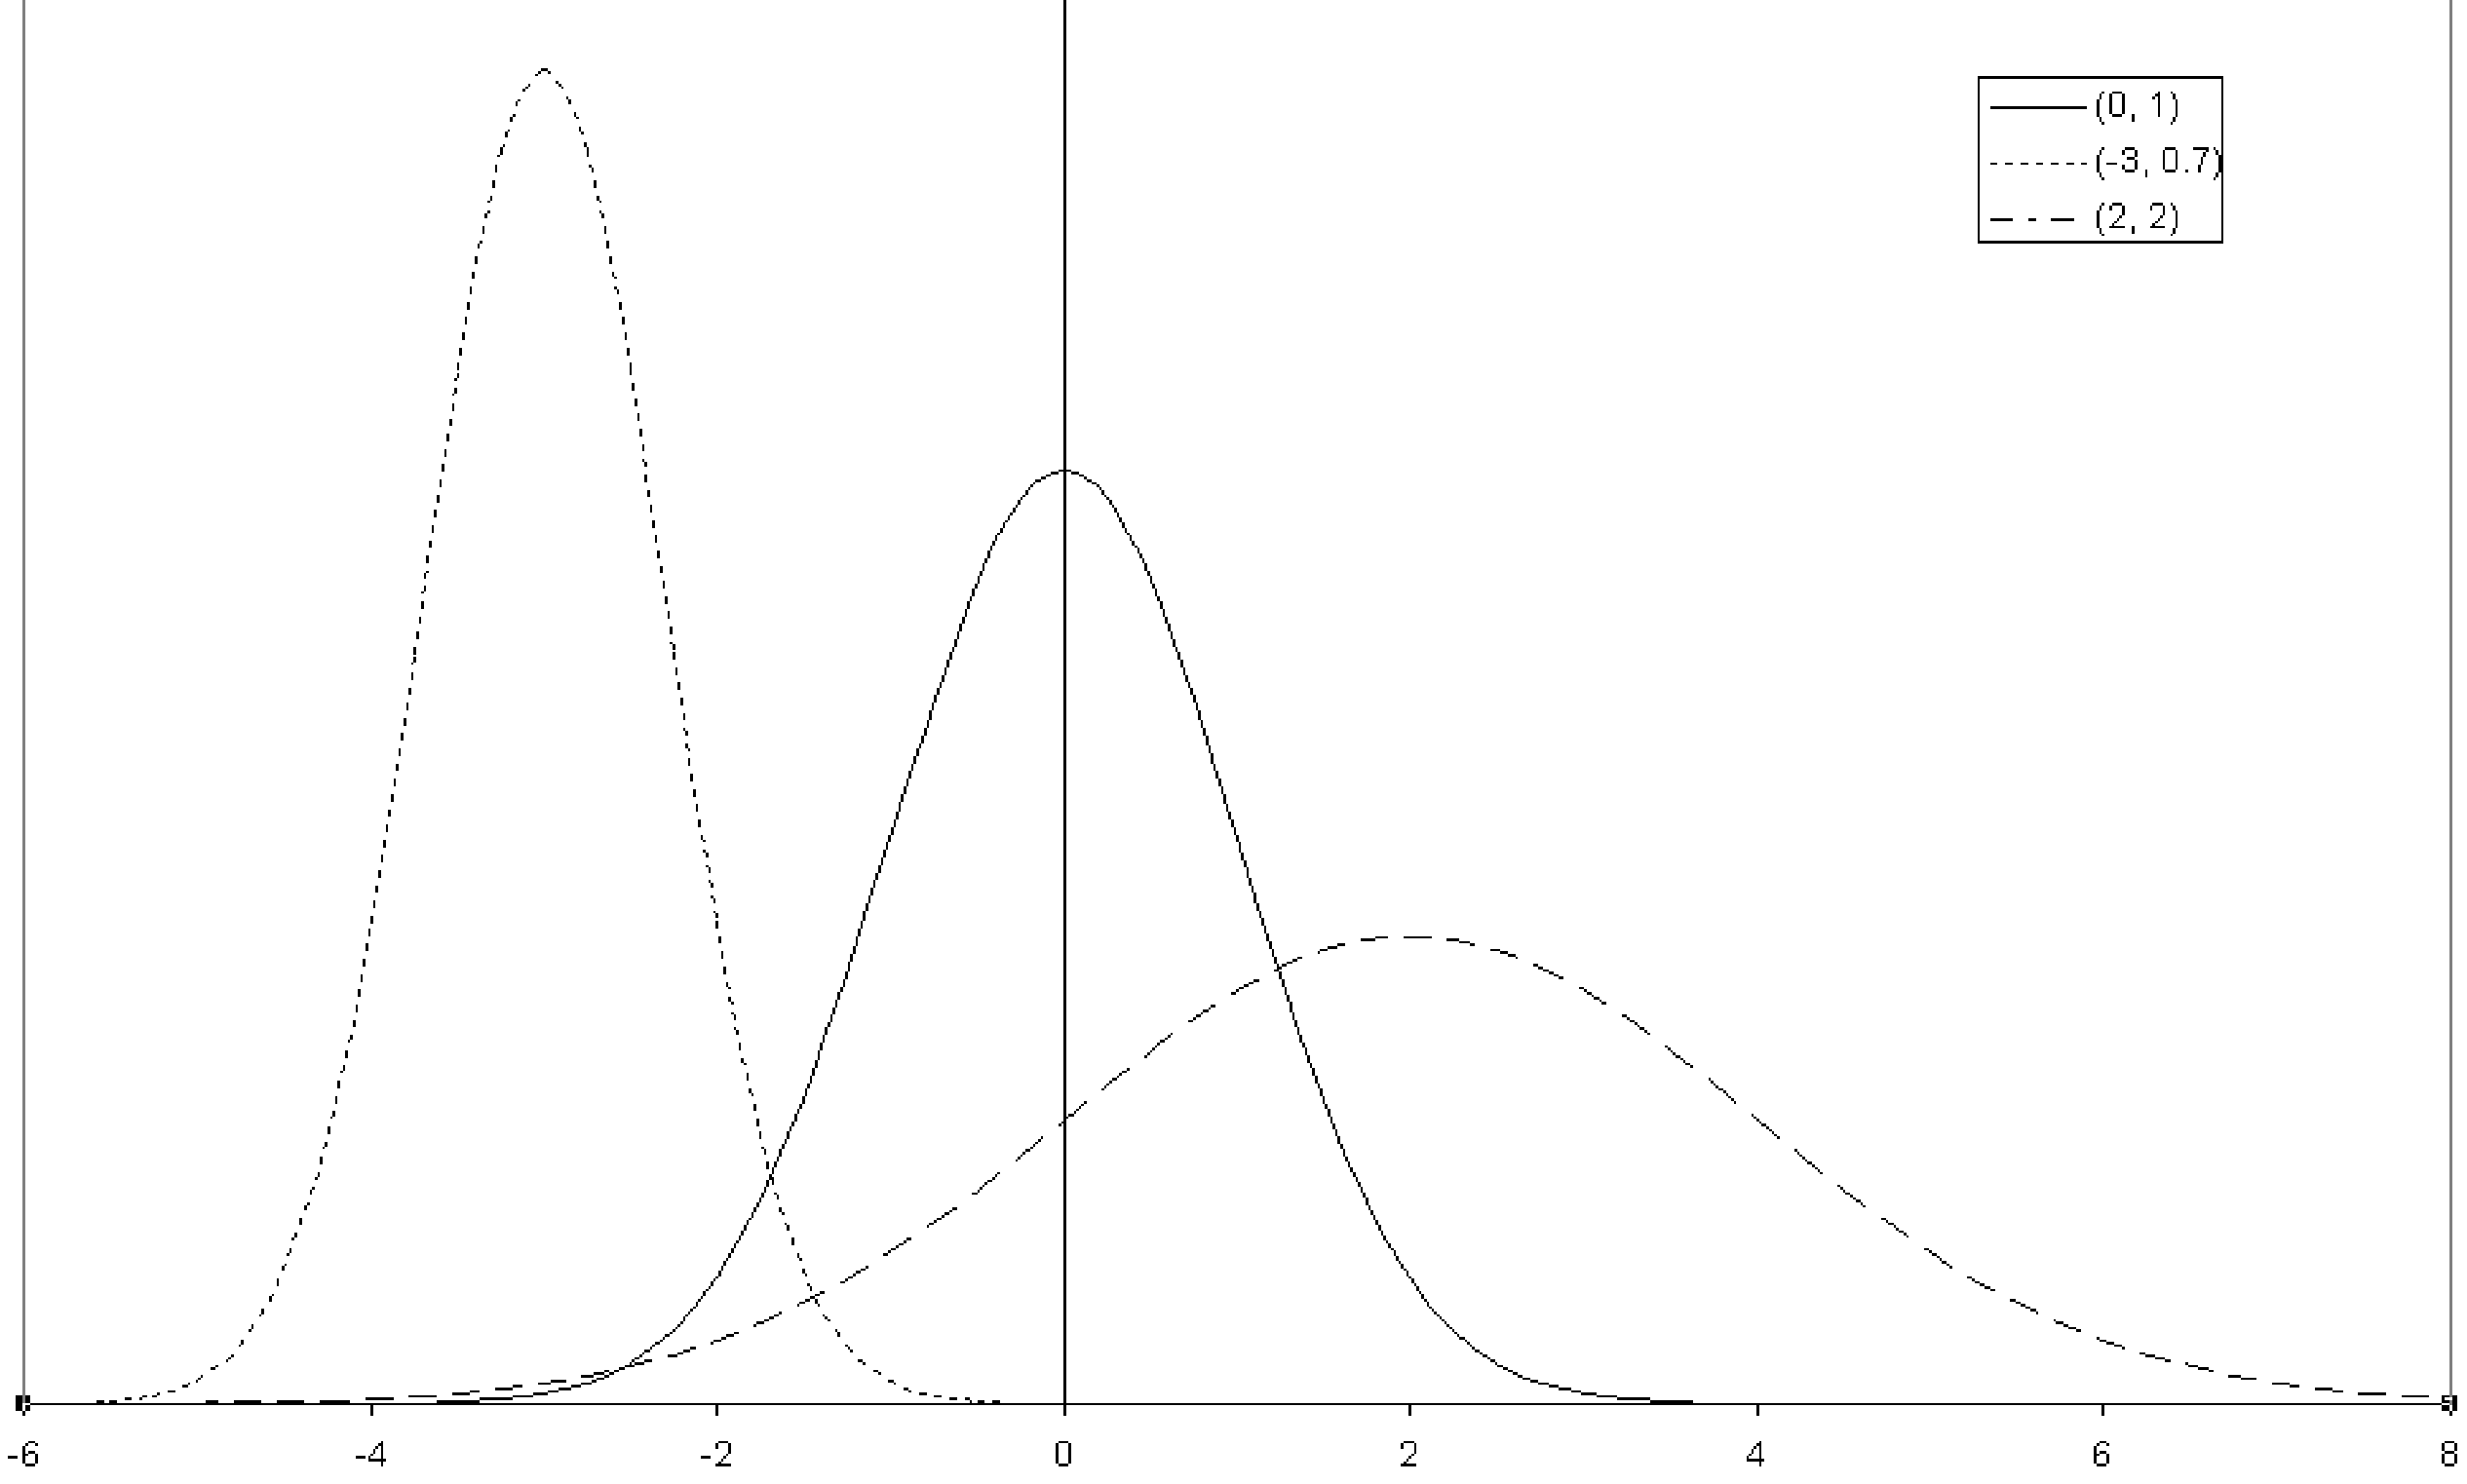
\includegraphics[width=12cm]{Figures/NormalDistribution}
\caption{Normal distribution for various values of the parameters
}\label{fig:normDistr}
\end{figure}

\subsection{Normal distribution --- Smalltalk implementation}
\marginpar{Figure \ref{fig:statisticsclasses} with the box {\textbf
NormalDistribution} grayed.} Listing \ref{ls:normdist} shows the
implementation of the normal distribution in Smalltalk.

The distribution function of the normal distribution can be
computed with the error function (\cf section
\ref{sec:errorFunction}). Therefore the class {\texttt
DhbNormalDistribution} is implemented as a subclass of {\texttt
DhbProbabilityDensity}.

\begin{listing} Smalltalk implementation of the normal distribution \label{ls:normdist}
$$\halign{ #\hfil&\quad#\hfil\cr {\sl Class}& {\Large\bf DhbNormalDistribution}\cr
{\sl Subclass of }&{\tt DhbProbabilityDensity}\cr\noalign{\vskip 1ex}

{\sl Instance variable names:}&\parbox[t]{4 in}{\tt  mu sigma nextRandom }\cr\noalign{\vskip 1ex}
{\sl Class variable names:}&\parbox[t]{4 in}{\tt  NextRandom }\cr\noalign{\vskip 1ex}}$$


Class methods
{\parskip 1ex\par\noindent}
{\bf distributionName}
\begin{verbatim}
    ^ 'Normal distribution'
\end{verbatim}
{\bf fromHistogram:} {\tt aHistogram}
\begin{verbatim}
    ^ self new: aHistogram average sigma: aHistogram standardDeviation
\end{verbatim}
{\bf new}
\begin{verbatim}
    ^self new: 0 sigma: 1
\end{verbatim}
{\bf new:} {\tt aNumber1} {\bf sigma:} {\tt aNumber2}
\begin{verbatim}
    ^ super new initialize: aNumber1 sigma: aNumber2
\end{verbatim}
{\bf random}
\begin{verbatim}
    | v1 v2 w y |
    NextRandom isNil
        ifTrue: [ [ v1 := Number random * 2 - 1.
                    v2 := Number random * 2 - 1.
                    w := v1 squared + v2 squared.
                    w > 1 ] whileTrue: [].
                  y := ( ( w ln * 2 negated) / w) sqrt.
                v1 := y * v1.
                NextRandom := y * v2.
                ]
        ifFalse:[ v1 :=NextRandom.
                  NextRandom := nil.
                ].
    ^ v1
\end{verbatim}

Instance methods
{\parskip 1ex\par\noindent}
{\bf average}
\begin{verbatim}
    ^ mu
\end{verbatim}
{\bf changeParametersBy:} {\tt aVector}
\begin{verbatim}
    mu := mu + ( aVector at: 1).
    sigma := sigma + ( aVector at: 2).
\end{verbatim}
{\bf distributionValue:} {\tt aNumber}
\begin{verbatim}
    ^ DhbErfApproximation new value: ( ( aNumber - mu) / sigma)
\end{verbatim}
{\bf initialize:} {\tt aNumber1} {\bf sigma:} {\tt aNumber2}
\begin{verbatim}
    mu := aNumber1.
    sigma := aNumber2.
    ^ self
\end{verbatim}
{\bf kurtosis}
\begin{verbatim}
    ^ 0
\end{verbatim}
{\bf parameters}
\begin{verbatim}
    ^Array with: mu with: sigma

\end{verbatim}
{\bf random}
\begin{verbatim}
    ^ self class random * sigma + mu
\end{verbatim}
{\bf skewness}
\begin{verbatim}
    ^ 0
\end{verbatim}
{\bf standardDeviation}
\begin{verbatim}
    ^ sigma
\end{verbatim}
{\bf value:} {\tt aNumber}
\begin{verbatim}
    ^ (DhbErfApproximation new normal: (aNumber - mu) / sigma) / 
                                                                 sigma
\end{verbatim}
{\bf valueAndGradient:} {\tt aNumber}
\begin{verbatim}
    | dp y |
    y := (aNumber - mu) / sigma.
    dp := (DhbErfApproximation new normal: y) / sigma.
    ^ Array with: dp
           with: ( DhbVector with: dp * y / sigma
                             with: dp * ( y squared - 1) / sigma)
\end{verbatim}


\end{listing}

\section{Gamma distribution}
\label{sec:gammadist} The gamma distribution is used to describe
the time between some task, for example the time between repairs.

The generalization of the gamma distribution to a range of the
random variable of the type $\left[x_{\min},+\infty\right[$ is
called a Pearson type III distribution. The average of a Pearson
type III distribution is $x_{\min}+\alpha\beta$. The central
moments are the same as those of the gamma distribution.

Table \ref{tb:gammadist} shows the properties of the gamma
distribution.
\begin{table}[h]
  \centering
  \caption{Properties of the gamma distribution}\label{tb:gammadist}
\vspace{1 ex}
\begin{tabular}{|l|c|} \hline
  \vbox to 3ex{}Range of random variable & $\left[0,+\infty\right[ $\\ *[1ex] \hline
  \vbox to 4ex{}Probability density function & $\displaystyle P\left(x\right)=
  {x^{\alpha - 1}\over \beta^{\alpha}\Gamma\left(\alpha\right)}e^{-{x\over\beta}}$ \\*[2ex]  \hline
  \vbox to 3ex{}Parameters & $0<\alpha<+\infty$ \\
  & $0<\beta<+\infty$\\*[1ex]  \hline
  \vbox to 4ex{}Distribution function & $\displaystyle F\left(x\right)=\Gamma\left({x\over\beta},\alpha\right)$ \\
  &(\cf section \ref{sec:incgamma}) \\*[1ex]  \hline
  \vbox to 3ex{}Average & $\alpha\beta$ \\*[1ex] \hline
  \vbox to 3ex{}Variance & $\alpha\beta^2$ \\*[1ex] \hline
  \vbox to 4ex{}Skewness & $\displaystyle{2\over\sqrt{\alpha}}$ \\*[2ex] \hline
  \vbox to 4ex{}Kurtosis & $\displaystyle{6\over\alpha}$ \\*[2ex] \hline
\end{tabular}
\end{table}
Figure \ref{fig:gammaDistr} shows the shape of the gamma
distribution for several values of the parameter $\alpha$ with
$\beta = 1$. The shape of the distribution for values of the
parameter $\beta$ can be obtained by modifying the scale of the
$x$-axis since $\beta$ is just a scale factor of the random
variable.
\begin{figure}
  \centering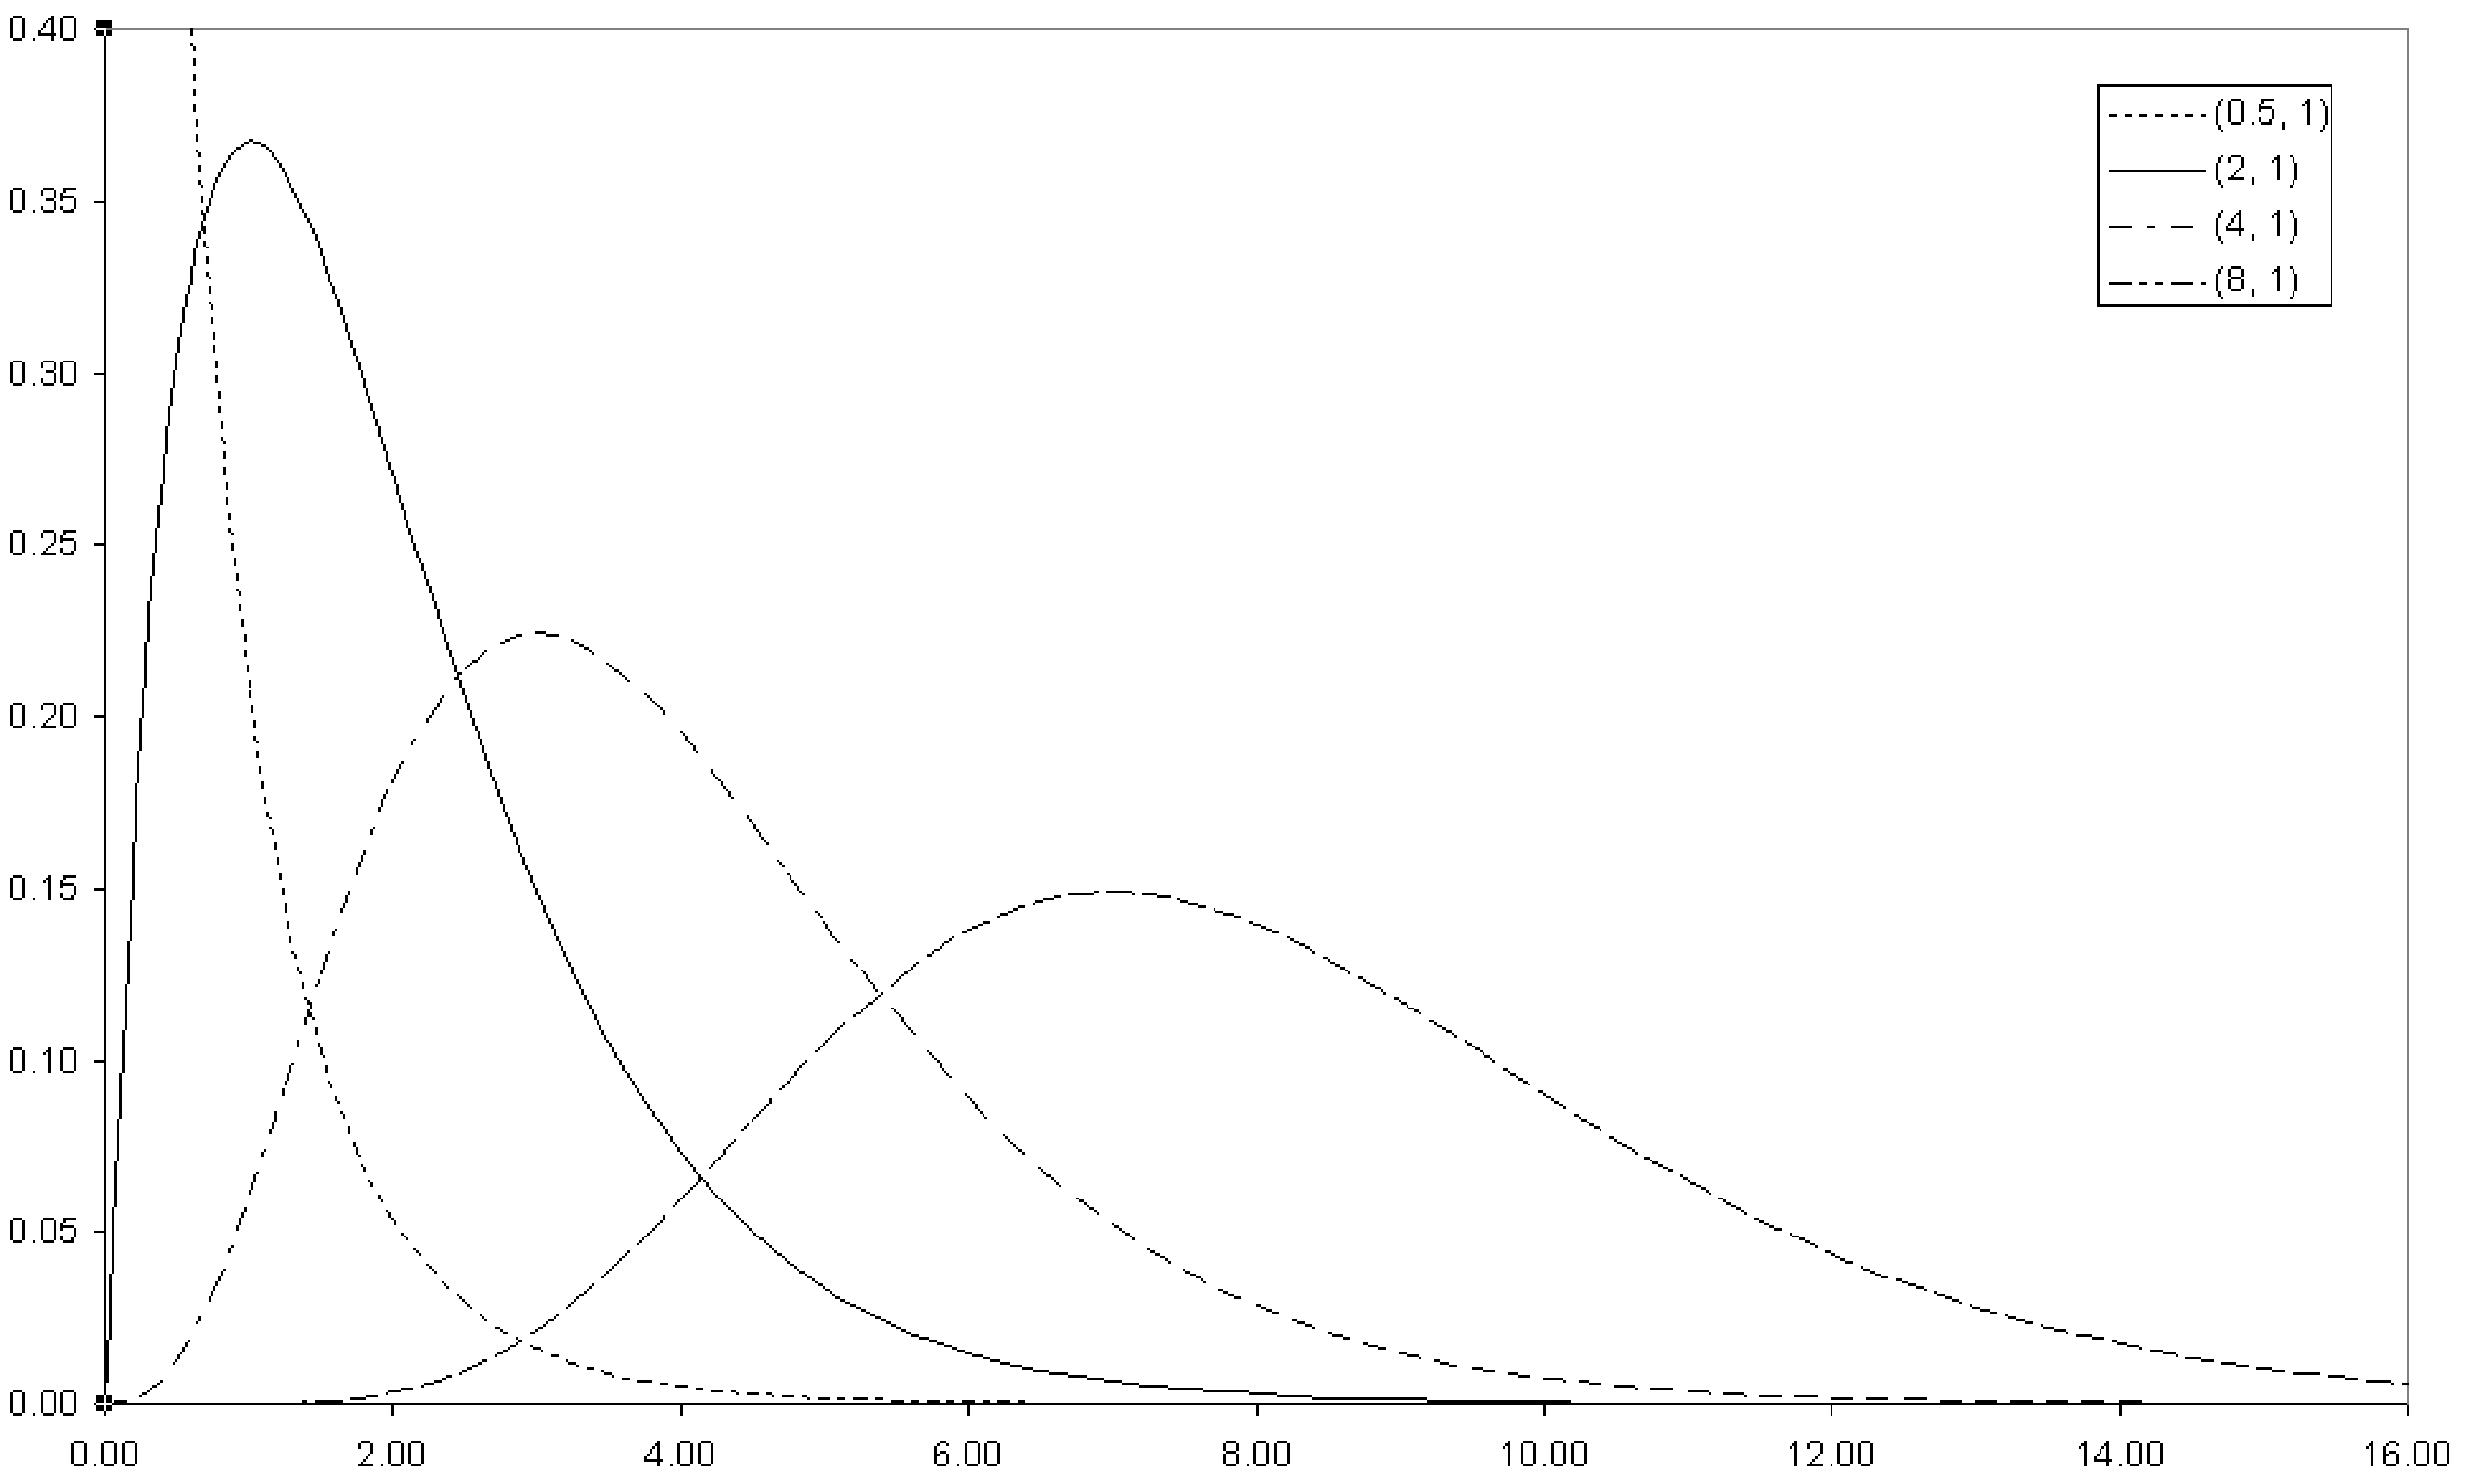
\includegraphics[width=12cm]{Figures/GammaDistribution}
  \caption{Gamma distribution for various values of $\alpha$
  }\label{fig:gammaDistr}
\end{figure}

\subsection{Gamma distribution --- Smalltalk implementation}
\label{sec:sgammadist}\marginpar{Figure
\ref{fig:statisticsclasses} with the box {\textbf GammaDistribution}
grayed.}  Listing \ref{ls:gammadist} shows the implementation of
the gamma distribution in Smalltalk.

The distribution function of the gamma distribution can be
computed with the incomplete gamma function (\cf section
\ref{sec:gammafunc}). Therefore the class {\texttt
DhbGammaDistribution} is implemented as a subclass of {\texttt
DhbProbabilityDensity}.
\begin{listing} Smalltalk implementation of the gamma distribution \label{ls:gammadist}
$$\halign{ #\hfil&\quad#\hfil\cr {\sl Class}& {\Large\bf DhbGammaDistribution}\cr
{\sl Subclass of }&{\tt DhbProbabilityDensity}\cr\noalign{\vskip 1ex}

{\sl Instance variable names:}&\parbox[t]{4 in}{\tt  alpha beta norm randomCoefficients incompleteGammaFunction }\cr\noalign{\vskip 1ex}}$$


Class methods
{\parskip 1ex\par\noindent}
{\bf distributionName}
\begin{verbatim}
    ^ 'Gamma distribution'
\end{verbatim}
{\bf fromHistogram:} {\tt aHistogram}
\begin{verbatim}
    | alpha beta |
    aHistogram minimum < 0
        ifTrue: [ ^nil].
    alpha := aHistogram average.
    beta := aHistogram variance / alpha.
    ^ [ self shape: alpha / beta scale: beta] when: ExAll do: [ 
                                       :signal | signal exitWith: nil]
\end{verbatim}
{\bf new}
\begin{verbatim}
    ^ self error: 'Illegal creation message for this class'
\end{verbatim}
{\bf shape:} {\tt aNumber1} {\bf scale:} {\tt aNumber2}
\begin{verbatim}
    ^ super new initialize: aNumber1 scale: aNumber2
\end{verbatim}

Instance methods
{\parskip 1ex\par\noindent}
{\bf average}
\begin{verbatim}
    ^ alpha * beta
\end{verbatim}
{\bf changeParametersBy:} {\tt aVector}
\begin{verbatim}
    alpha := alpha + ( aVector at: 1).
    beta := beta + ( aVector at: 2).
    self computeNorm.
    incompleteGammaFunction := nil.
    randomCoefficients := nil.
\end{verbatim}
{\bf computeNorm}
\begin{verbatim}
    norm := beta ln * alpha + alpha logGamma.
\end{verbatim}
{\bf distributionValue:} {\tt aNumber}
\begin{verbatim}
    ^ self incompleteGammaFunction value: aNumber / beta
\end{verbatim}
{\bf incompleteGammaFunction}
\begin{verbatim}
    incompleteGammaFunction isNil 
        ifTrue: 
            [ incompleteGammaFunction := DhbIncompleteGammaFunction 
                                                        shape: alpha ].
    ^ incompleteGammaFunction
\end{verbatim}
{\bf initialize:} {\tt aNumber1} {\bf scale:} {\tt aNumber2}
\begin{verbatim}
    (aNumber1 > 0 and: [ aNumber2 > 0])
        ifFalse: [ self error: 'Illegal distribution parameters'].
    alpha := aNumber1.
    beta := aNumber2.
    self computeNorm.
    ^ self
\end{verbatim}
{\bf initializeRandomCoefficientsForLargeAlpha}
\begin{verbatim}
    | a b q d |
    a := 1 / ( 2 * alpha - 1) sqrt.
    b := alpha - (4 ln).
    q := 1 / a + alpha.
    d := 4.5 ln + 1.
    ^ Array with: a with: b with: q with: d
\end{verbatim}
{\bf initializeRandomCoefficientsForSmallAlpha}
\begin{verbatim}
    | e |
    e := 1 exp.
    ^ (e + alpha) / e
\end{verbatim}
{\bf kurtosis}
\begin{verbatim}
    ^ 6 / alpha
\end{verbatim}
{\bf parameters}
\begin{verbatim}
    ^ Array with: alpha with: beta
\end{verbatim}
{\bf random}
\begin{verbatim}
    ^ ( alpha > 1 ifTrue: [ self randomForLargeAlpha]
                        ifFalse:[ self randomForSmallAlpha]) * beta
\end{verbatim}
{\bf randomCoefficientsForLargeAlpha}
\begin{verbatim}
    randomCoefficients isNil
        ifTrue: [ randomCoefficients := self initializeRandomCoefficientsForLargeAlpha].
    ^ randomCoefficients
\end{verbatim}
{\bf randomCoefficientsForSmallAlpha}
\begin{verbatim}
    randomCoefficients isNil
        ifTrue: [ randomCoefficients := self 
                           initializeRandomCoefficientsForSmallAlpha].
    ^ randomCoefficients
\end{verbatim}
{\bf randomForLargeAlpha}
\begin{verbatim}
    [ true] whileTrue: [
    | u1 u2 c v y z w |
    u1 := DhbMitchellMooreGenerator new floatValue.
    u2 := DhbMitchellMooreGenerator new floatValue.
    c := self randomCoefficientsForLargeAlpha.
    v := ( u1 / ( 1 - u1)) ln * (c at: 1).
    y := v exp * alpha.
    z := u1 squared * u2.
    w := ( c at: 3) * v + ( c at: 2) - y.
    ( c at: 4) + w >= ( 4.5 * z) ifTrue: [ ^y].
    z ln <= w ifTrue: [ ^y].
    ].
\end{verbatim}
{\bf randomForSmallAlpha}
\begin{verbatim}
    [ true] whileTrue: [
    | p |
    p := DhbMitchellMooreGenerator new floatValue * self 
                                      randomCoefficientsForSmallAlpha.
    p > 1
        ifTrue: [ | y |
                     y := ( ( self randomCoefficientsForSmallAlpha - 
                                               p) / alpha) ln negated.
                     DhbMitchellMooreGenerator new floatValue <= ( y 
                                               raisedTo: ( alpha - 1))
                        ifTrue: [ ^y].
                    ]
        ifFalse: [ | y |
                        y := p raisedTo: ( 1 / alpha).
                     DhbMitchellMooreGenerator new floatValue <= ( y 
                                                          negated exp)
                        ifTrue: [ ^y].
                     ].
    ].
\end{verbatim}
{\bf skewness}
\begin{verbatim}
    ^ 2 / alpha sqrt
\end{verbatim}
{\bf value:} {\tt aNumber}
\begin{verbatim}
    ^ aNumber > 0
        ifTrue: [ ( aNumber ln * (alpha - 1) - (aNumber / beta) - 
                                                            norm) exp ]
        ifFalse:[ 0 ].
\end{verbatim}
{\bf variance}
\begin{verbatim}
    ^ beta squared * alpha
\end{verbatim}


\end{listing}


\section{Experimental distribution}
A histogram described in section \ref{sec:histogram} can be used
as a probability distribution. After all, a histogram can be
considered as the representation of a distribution, which has been
measured experimentally.

If $N$ is the total count of the histogram and $n_i$ the count in
bin number $i$ the probability of finding a measurement within the
bin number $i$ is simply given by:
\begin{equation}
  P_i={\displaystyle n_i \over\displaystyle N}.
\end{equation}
If $w$ is the width of each bin, the probability density function
of the distribution measured by the histogram can be estimated by:
\begin{equation}
\label{eq:histprob}
  P\left(x\right)={\displaystyle P_i \over\displaystyle w}
  ={\displaystyle n_i \over\displaystyle wN}\mbox{\quad
  where $i=\left\lfloor{\displaystyle x-x_{\min}\over\displaystyle w}\right\rfloor$.}
\end{equation}
Equation \ref{eq:histprob} is only valid for $x_{\min}\le x <
x_{\max}$. Outside of the histogram's limits there is no
information concerning the shape of the probability density
function.

The distribution function is computed by evaluating the sum of all
bins located below the argument and by adding a correction
computed by linear interpolation over the bin in which the value
is located. Thus, we have:
\begin{equation}
\label{eq:histdistr}
  F\left(x\right)={\displaystyle 1 \over\displaystyle N} \left(\sum_{j=1}^{i-1}n_j
  + {x-x_i \over w}n_i\right)
  \mbox{\quad where $i=\left\lfloor{\displaystyle x-x_{\min}\over\displaystyle w}\right\rfloor$.}
\end{equation}
If $x<x_{\min}$, $F\left(x\right)=0$ and if $x\geq x_{\max}$,
$F\left(x\right)=1$. A similar equation can be derived for the
acceptance interval function.

\subsection{Experimental distribution --- General  implementation}
\marginpar{Figure \ref{fig:statisticsclasses} with the box {\textbf
HistogrammedDistribution} grayed.} Adding the responsibility of
behaving like a probability density function to a histogram is not
desirable. In a good object oriented design, objects should have
only one responsibility or type of behavior.

Thus, a good object oriented implementation implements an
\patstyle{Adapter} pattern. One creates an object, having the
behavior of a probability density function. A single instance
variable inside this object refers to the histogram, over which
the experimental distribution is defined. The \patstyle{Adapter}
object is a subclass of the abstract class describing all
probability density functions.

The parameters of the distribution --- average, variance, skewness
and kurtosis --- are obtained from the histogram itself.

The computation of the distribution and the interval acceptance
function is delegated to the histogram. The floor operation of
equation \ref{eq:histdistr} is evaluated by the method {\texttt
binIndex} of the histogram.

\begin{quote}
{\textbf Note:} In both implementation, there is no protection against
illegal arguments. Illegal arguments can occur when computing the
distribution value when the histogram underflow and overflow
counts are non zero. Below the minimum and above the maximum, no
information can be obtained for the distribution. Within the
histogram limits, there is no need for protection. Therefore the
implementation assumes that the histogram was collected using
automatic adjustment of the limits (\cf section
\ref{sec:histogram}).
\end{quote}

\subsection{Experimental distribution --- Smalltalk  implementation}
Listing \ref{ls:histprob} shows the implementation of an
experimental distribution in Smalltalk.

The class {\texttt DhbHistogrammedDistribution} is a subclass of the
class {\texttt DhbProbabilityDensity}. The class creation method {\texttt
histogram:} takes as argument the histogram over which the
instance is defined. To prevent creating a instance with undefined
instance variable, the default class creation method {\texttt new}
returns an error.

\begin{listing} Smalltalk implementation of an experimental distribution \label{ls:histprob}
$$\halign{ #\hfil&\quad#\hfil\cr {\sl Class}& {\Large\bf DhbHistogrammedDistribution}\cr
{\sl Subclass of }&{\tt DhbProbabilityDensity}\cr\noalign{\vskip 1ex}

{\sl Instance variable names:}&\parbox[t]{4 in}{\tt  histogram }\cr\noalign{\vskip 1ex}}$$


Class methods
{\parskip 1ex\par\noindent}
{\bf distributionName}
\begin{verbatim}
    ^ 'Experimental distribution'
\end{verbatim}
{\bf histogram:} {\tt aHistogram}
\begin{verbatim}
    ^ super new initialize: aHistogram
\end{verbatim}
{\bf new}
\begin{verbatim}
    ^ self error: 'Illegal creation message for this class'
\end{verbatim}

Instance methods
{\parskip 1ex\par\noindent}
{\bf acceptanceBetween:} {\tt aNumber1} {\bf and:} {\tt aNumber2}
\begin{verbatim}
    ^ (histogram countsBetween: (aNumber1 max: histogram minimum)
                        and: (aNumber2 min: histogram maximum) ) / 
                                                  histogram totalCount

\end{verbatim}
{\bf average}
\begin{verbatim}
    ^ histogram average

\end{verbatim}
{\bf distributionValue:} {\tt aNumber}
\begin{verbatim}
    ^ aNumber < histogram minimum
        ifTrue: [ 0 ]
        ifFalse:[ aNumber < histogram maximum
                            ifTrue: [ ( histogram countsUpTo: 
                                      aNumber) / histogram totalCount ]
                            ifFalse:[ 1 ]
                    ]
\end{verbatim}
{\bf initialize:} {\tt aHistogram}
\begin{verbatim}
    aHistogram count = 0
        ifTrue: [ self error: 'Cannot define probability density on 
                                                 an empty histogram'].
    histogram := aHistogram.
    ^ self
\end{verbatim}
{\bf kurtosis}
\begin{verbatim}
    ^ histogram kurtosis
\end{verbatim}
{\bf privateInverseDistributionValue:} {\tt aNumber}
\begin{verbatim}
    ^ histogram inverseDistributionValue: aNumber
\end{verbatim}
{\bf skewness}
\begin{verbatim}
    ^ histogram skewness
\end{verbatim}
{\bf standardDeviation}
\begin{verbatim}
    ^ histogram standardDeviation
\end{verbatim}
{\bf value:} {\tt aNumber}
\begin{verbatim}
    ^ (aNumber >= histogram minimum and: [ aNumber < histogram 
                                                             maximum])
        ifTrue: [ ( histogram countAt: aNumber) / ( histogram 
                                     totalCount * histogram binWidth)]
        ifFalse:[ 0 ]
\end{verbatim}
{\bf variance}
\begin{verbatim}
    ^ histogram variance
\end{verbatim}


\end{listing}


%\ifx\wholebook\relax\else\end{document}\fi
